% !Tex root=tb_icml_2018.tex

\section{Additional Empirical Analysis of SNR}
\label{sec:app:emp}

\subsection{Histograms for VAE}
\label{sec:hist-vae}

To complete the picture for the effect of $M$ and $K$ on the distribution
of the gradients, we generated histograms for the $K=1$ (i.e. \gls{VAE})
gradients as $M$ is varied.  As shown in Figure~\ref{fig:snr/b_hist_vae},
we see the expected effect from the law of large numbers that the 
variance of the estimates decreases with $M$, but not the expected value.

\begin{figure*}[h]
	\centering
%	\begin{subfigure}[b]{0.49\textwidth}
%		\centering
%		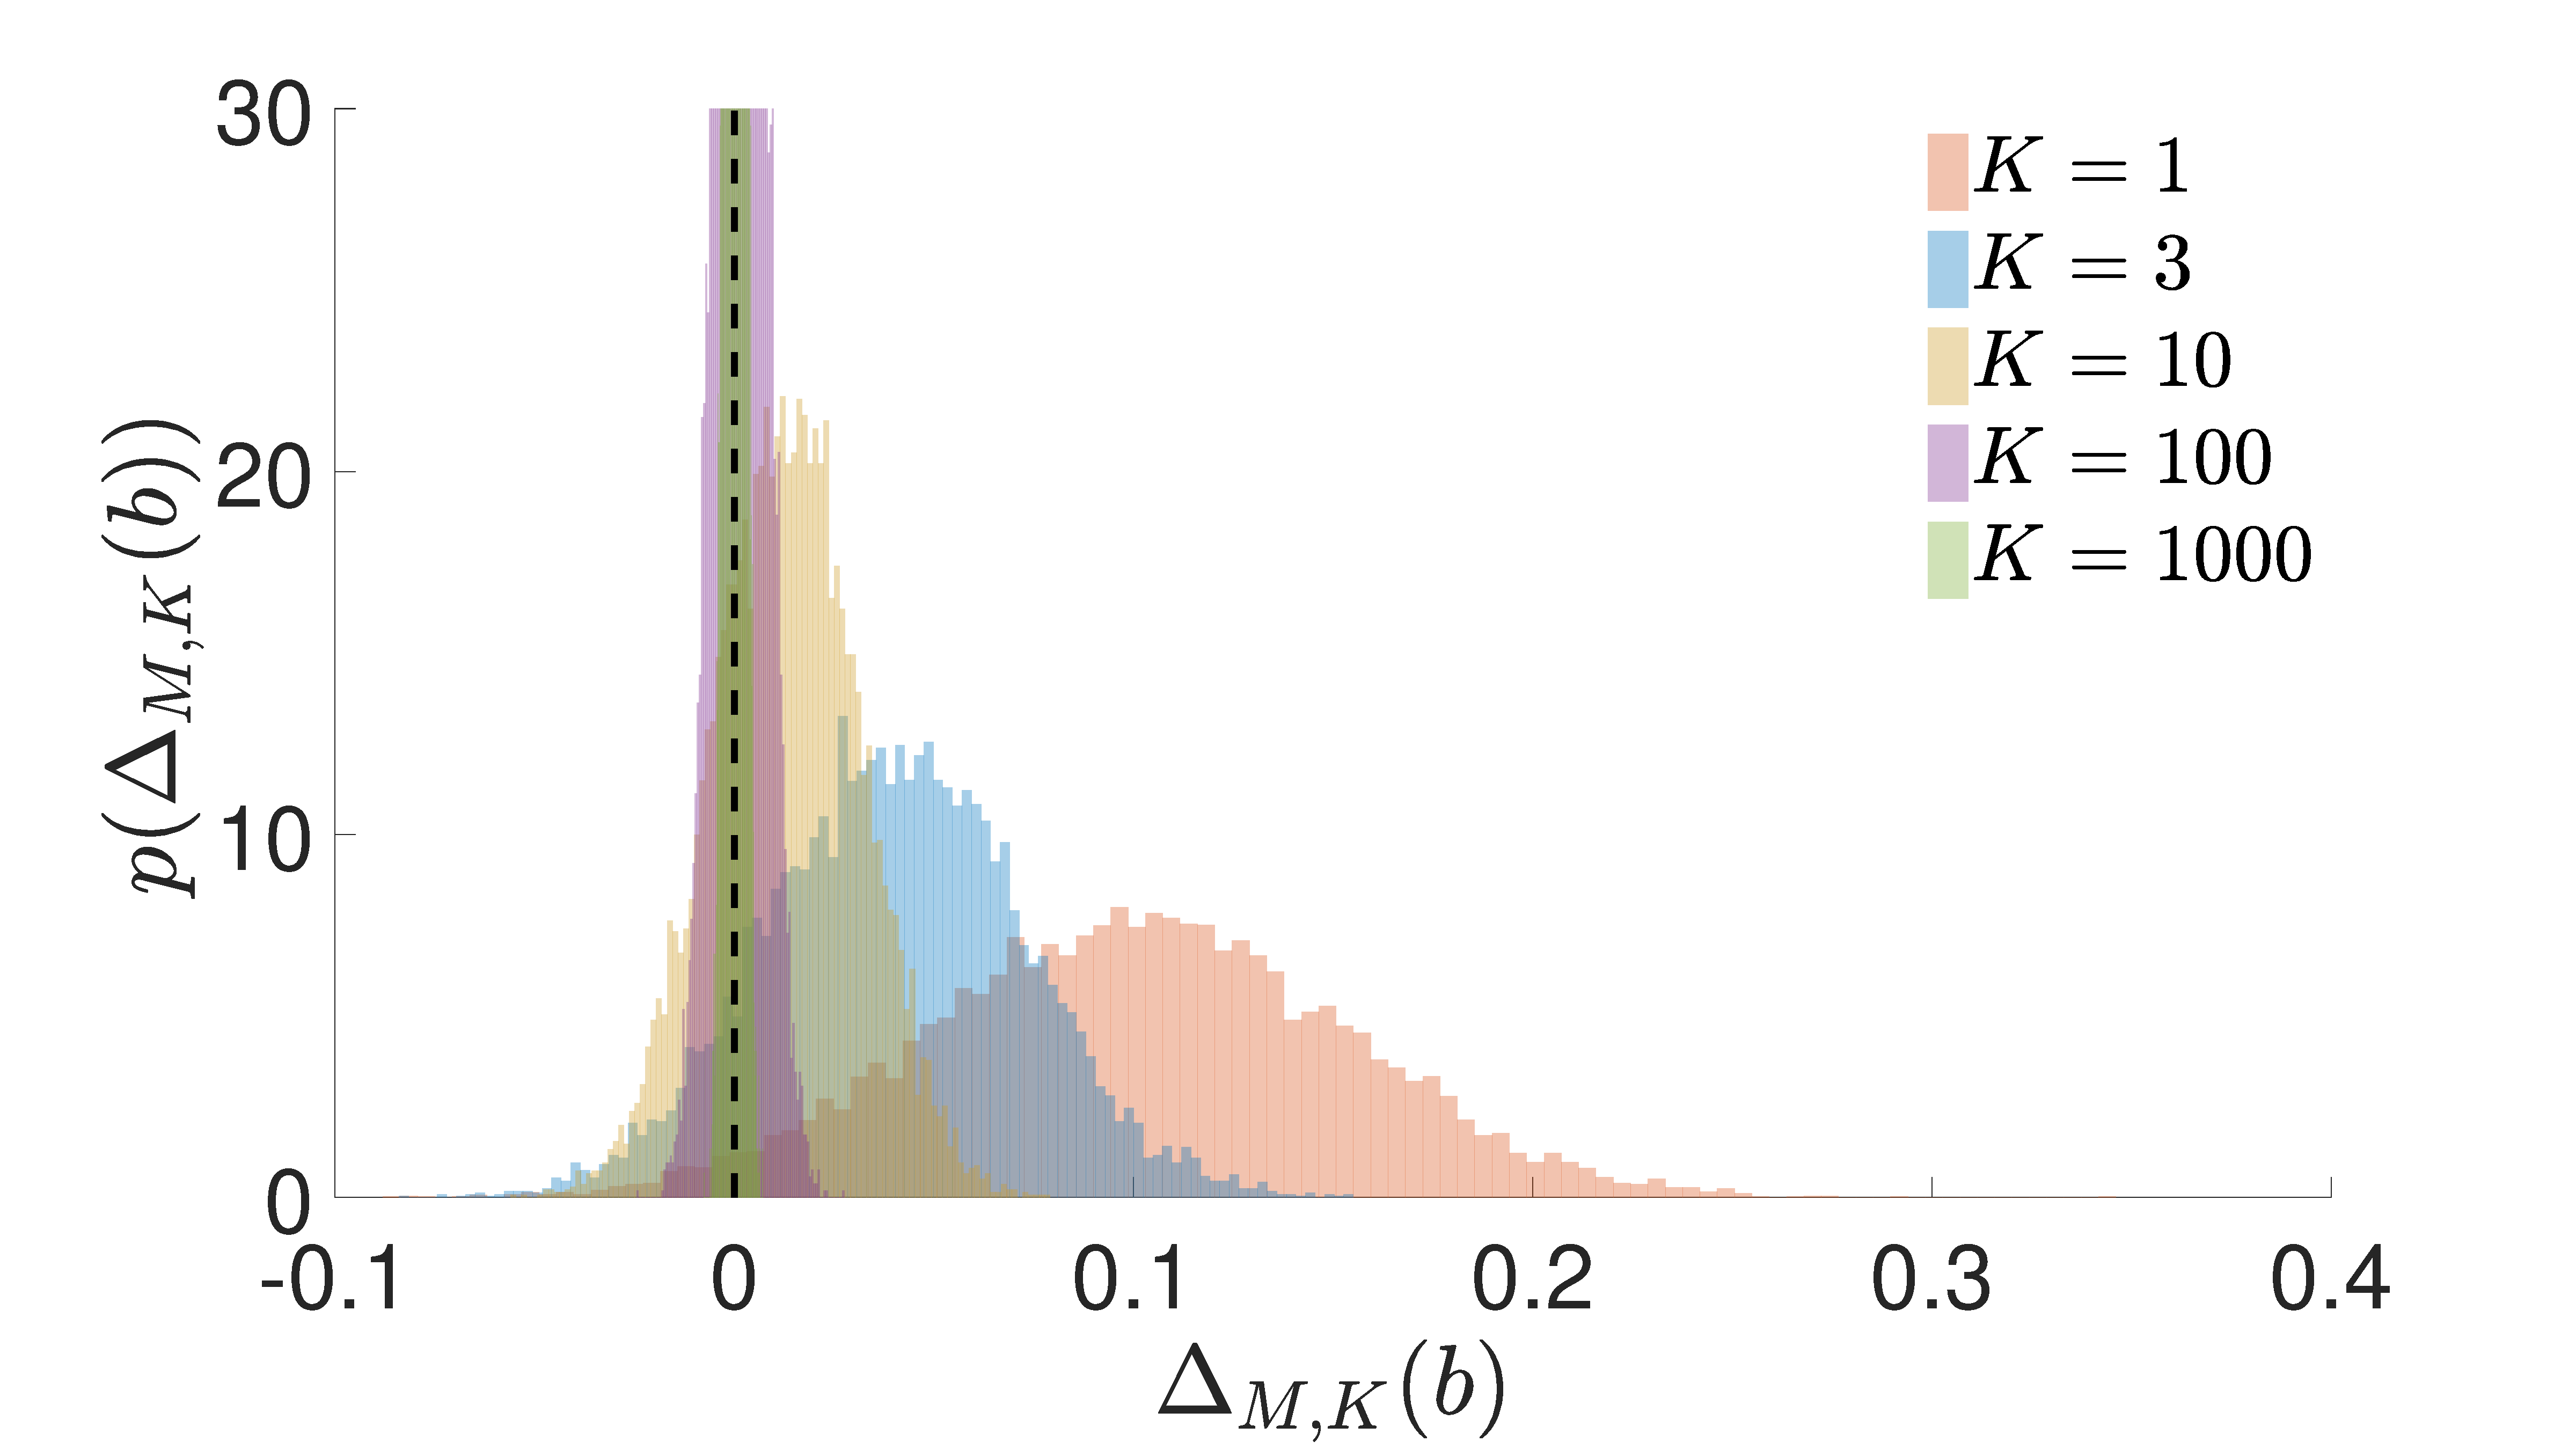
\includegraphics[width=\textwidth]{b_hist_IWAE}
%		\caption{\gls{IWAE} inference network gradient estimates \label{fig:snr/b_hist_iwae}}
%	\end{subfigure}
		\begin{subfigure}[b]{0.45\textwidth}
			\centering
			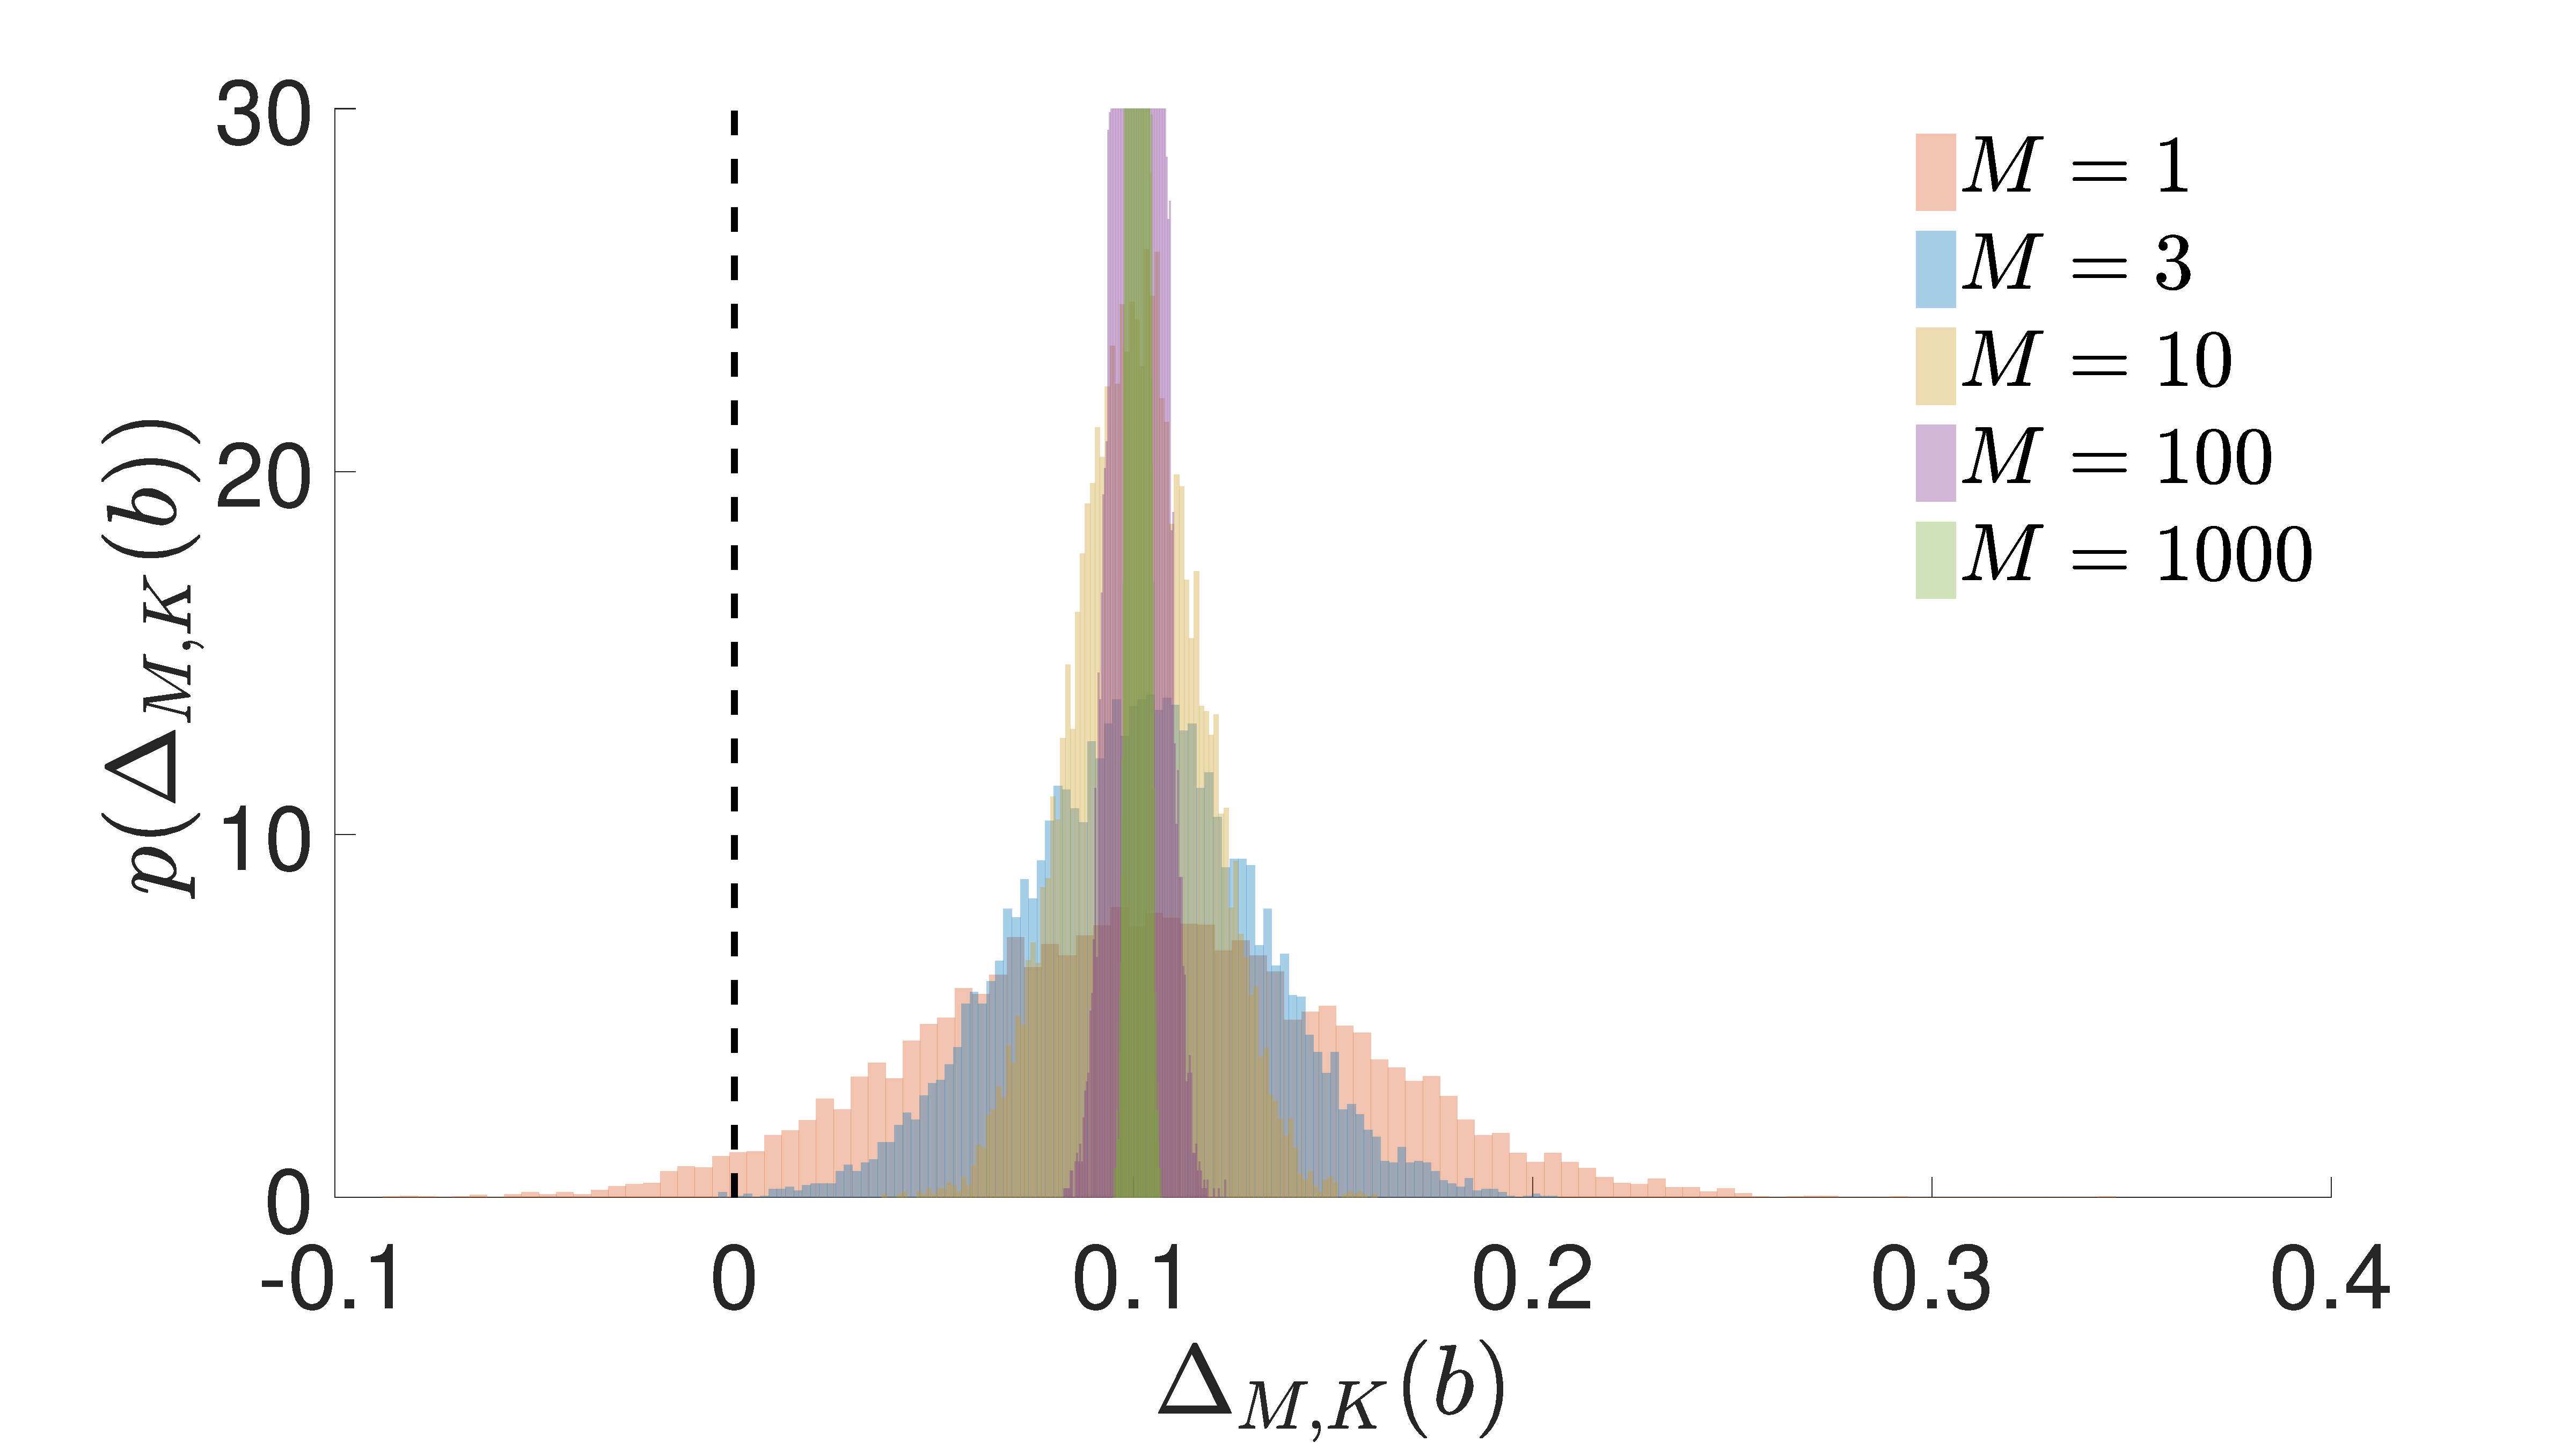
\includegraphics[width=\textwidth]{b_hist_VAE}
			\caption{\gls{VAE} inference network gradient estimates \label{fig:snr/b_hist_vae}}
		\end{subfigure} ~~~~~~~~~~
%	\begin{subfigure}[b]{0.49\textwidth}
%		\centering
%		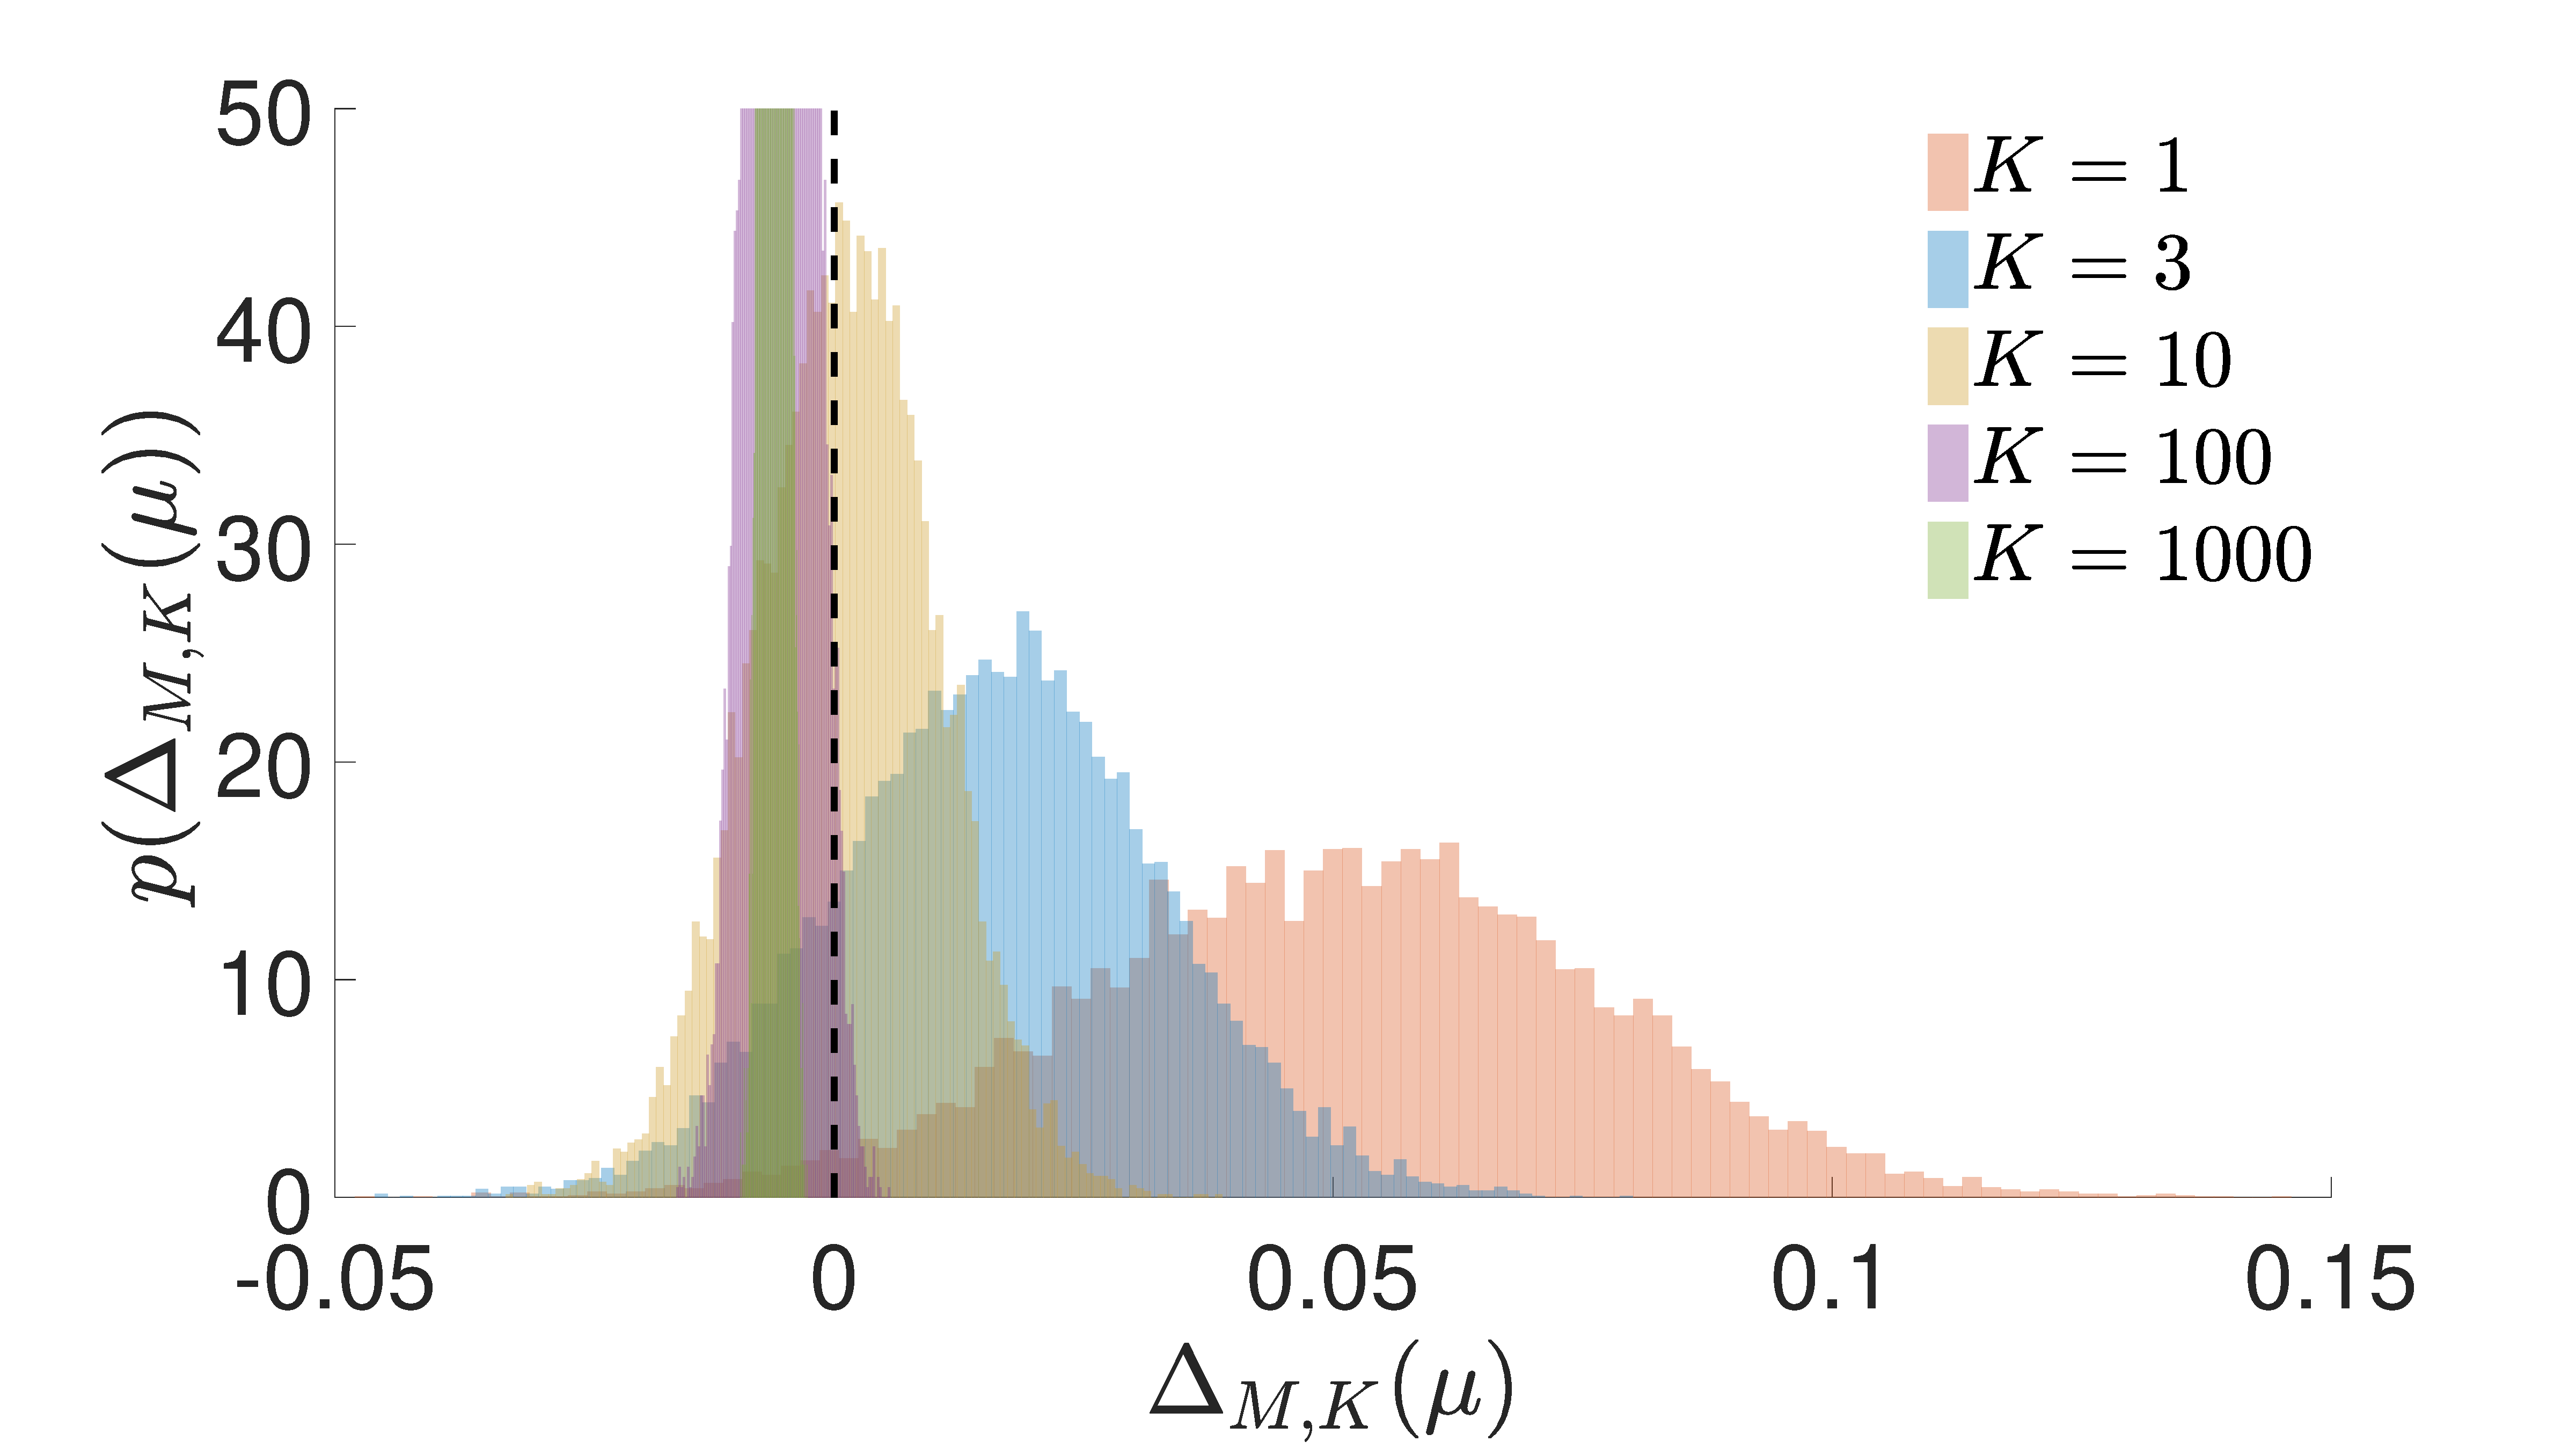
\includegraphics[width=\textwidth]{mu_hist_IWAE}
%		\caption{\gls{IWAE} generative network gradient estimates \label{fig:snr/mu_hist_iwae}}
%	\end{subfigure}
		\begin{subfigure}[b]{0.45\textwidth}
			\centering
			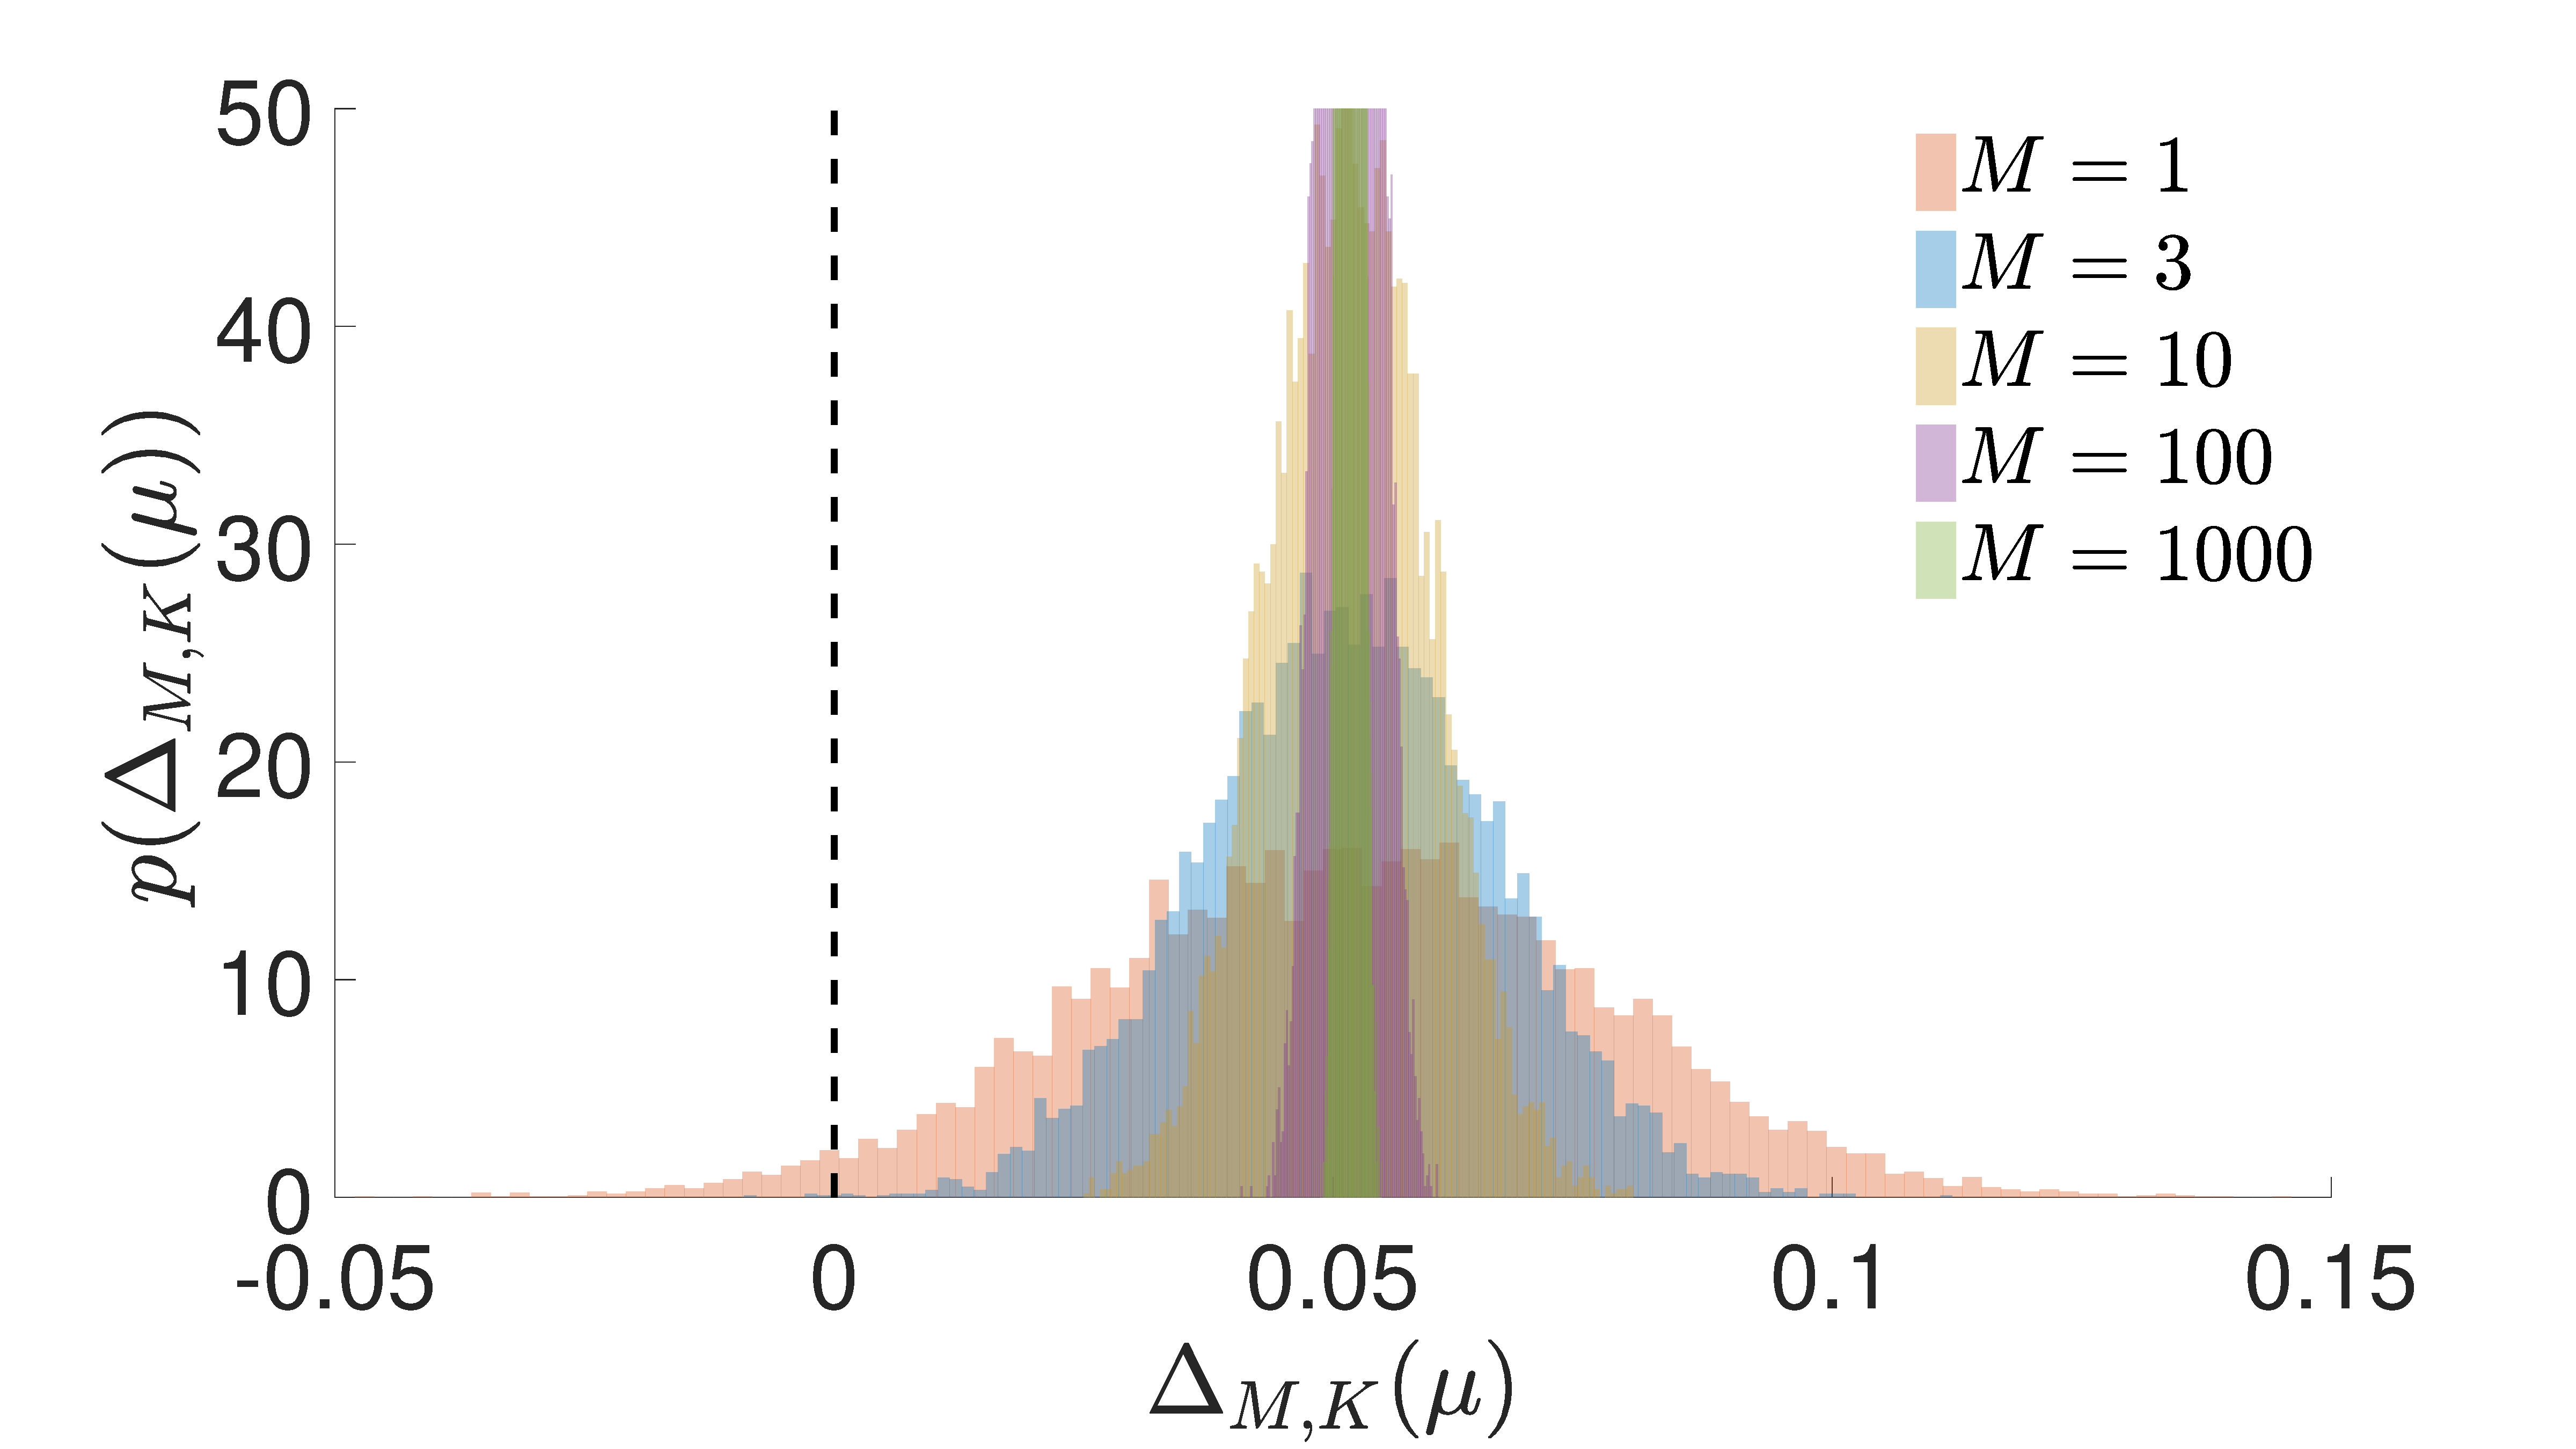
\includegraphics[width=\textwidth]{mu_hist_VAE}
			\caption{\gls{VAE} generative network gradient estimates \label{fig:snr/mu_hist_vae}}
		\end{subfigure}
	\caption{Histograms of gradient estimates $\Delta_{M,K}$ for the generative network and 
		the	inference network using the \gls{VAE} ($K=1$) objectives with different values of $M$. \vspace{-12pt}
		\label{fig:snr/hists-vae}}
\end{figure*}

\subsection{Convergence of RMSE for Generative Network}
\label{sec:app:rmse}

\begin{wrapfigure}{r}{0.5\textwidth}
	\centering
	\vspace{-15pt}
	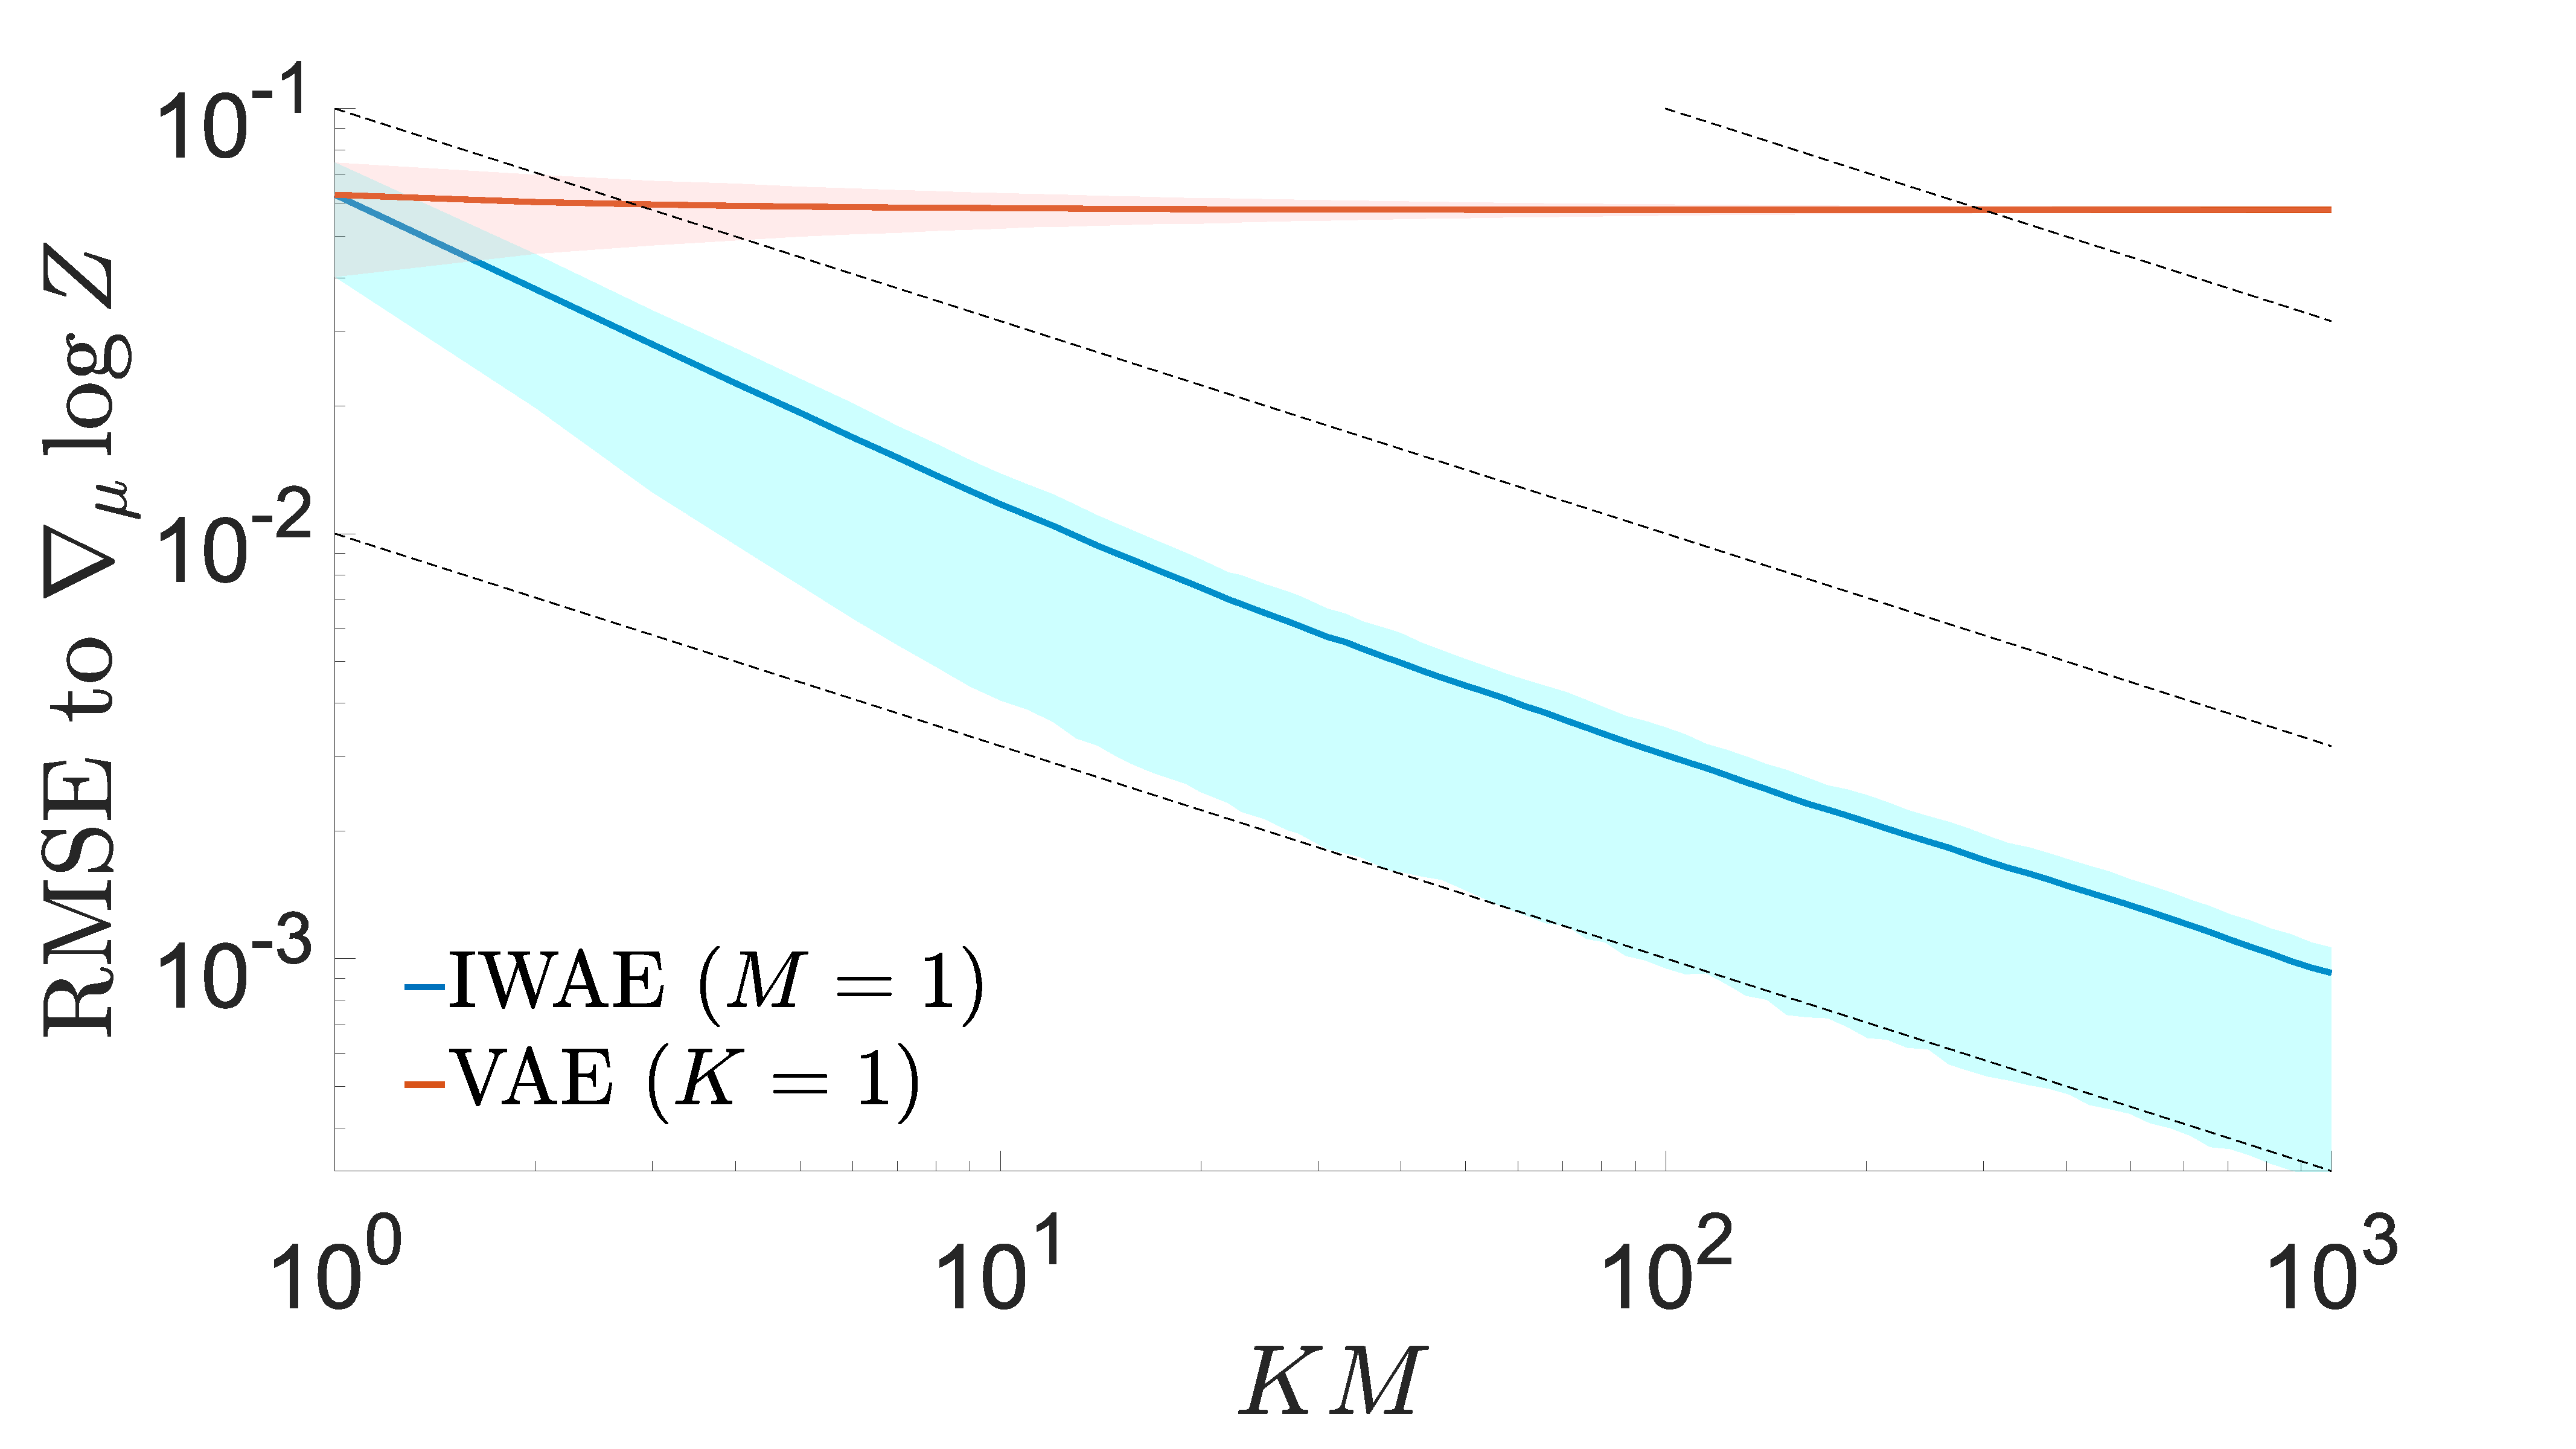
\includegraphics[width=0.47\textwidth]{mse_mu}
	\vspace{-10pt}
	\caption{RMSE in $\mu$ gradient estimate to $\nabla_{\mu} \log Z$ 
		\label{fig:snr/rmse}}
	\vspace{-8pt}
\end{wrapfigure} 
As explained in the main paper, the SNR is not an entirely appropriate metric for
the generative network -- a low SNR is still highly problematic, but a high SNR
does not indicate good performance.
It is thus perhaps better to measure
the quality of the gradient estimates for the generative network by looking at the \gls{RMSE}
to $\nabla_{\mu} \log Z$, i.e. $\sqrt{\E \left[\lVert\Delta_{M,K}-\nabla_{\mu} \log Z\rVert_2^2\right]}$.
The convergence of this \gls{RMSE}  is shown in
Figure~\ref{fig:snr/rmse} where the solid lines are the \gls{RMSE} estimates using $10^4$ runs 
and the shaded regions
show the interquartile range of the individual estimates. We see that increasing 
$M$ in the \gls{VAE} reduces the variance
of the estimates but has negligible effect on the \gls{RMSE} due to the fixed bias.  On the
other hand,
we see that increasing $K$ leads to a monotonic improvement, initially improving
at a rate $O(1/K)$ (because the bias is the dominating term in this region),
before settling to the standard Monte Carlo convergence rate of $O(1/\sqrt{K})$
(shown by the dashed lines).

\subsection{Experimental Results for High Variance Regime}
\label{sec:hv}

\vspace{-4pt}

We now present empirical results for a case where our weights are higher variance. Instead
of choosing a point close to the optimum by offsetting parameters with a standard deviation of $0.01$, 
we instead offset using a standard deviation of $0.5$.  We further increased the proposal covariance to $I$
to make it more diffuse.  This is now a scenario where the model is far from its optimum and the proposal
is a very poor match for the model, giving very high variance weights.


We see that the behavior is the
same for variation in $M$, but somewhat distinct for variation in $K$.  
In particular, the \gls{SNR} and \textsc{dsnr} only decrease slowly with $K$ for the inference network, while increasing $K$ no longer has much benefit for the \gls{SNR} of the
inference network.
%Increasing $K$ now also has a remarkably similar impact on the \gls{SNR} and \textsc{dsnr} of
%the gradients of the generative network as on the
%inference network.  
It is clear that, for this
setup, the problem is very far from the asymptotic regime in $K$ such that our theoretical results no
longer directly apply.  Nonetheless, the high-level effect observed is still that the \gls{SNR} of 
the inference
network deteriorates, albeit slowly, as $K$ increases.

\begin{figure}[h]
	\centering
	\begin{subfigure}[b]{0.45\textwidth}
		\centering
		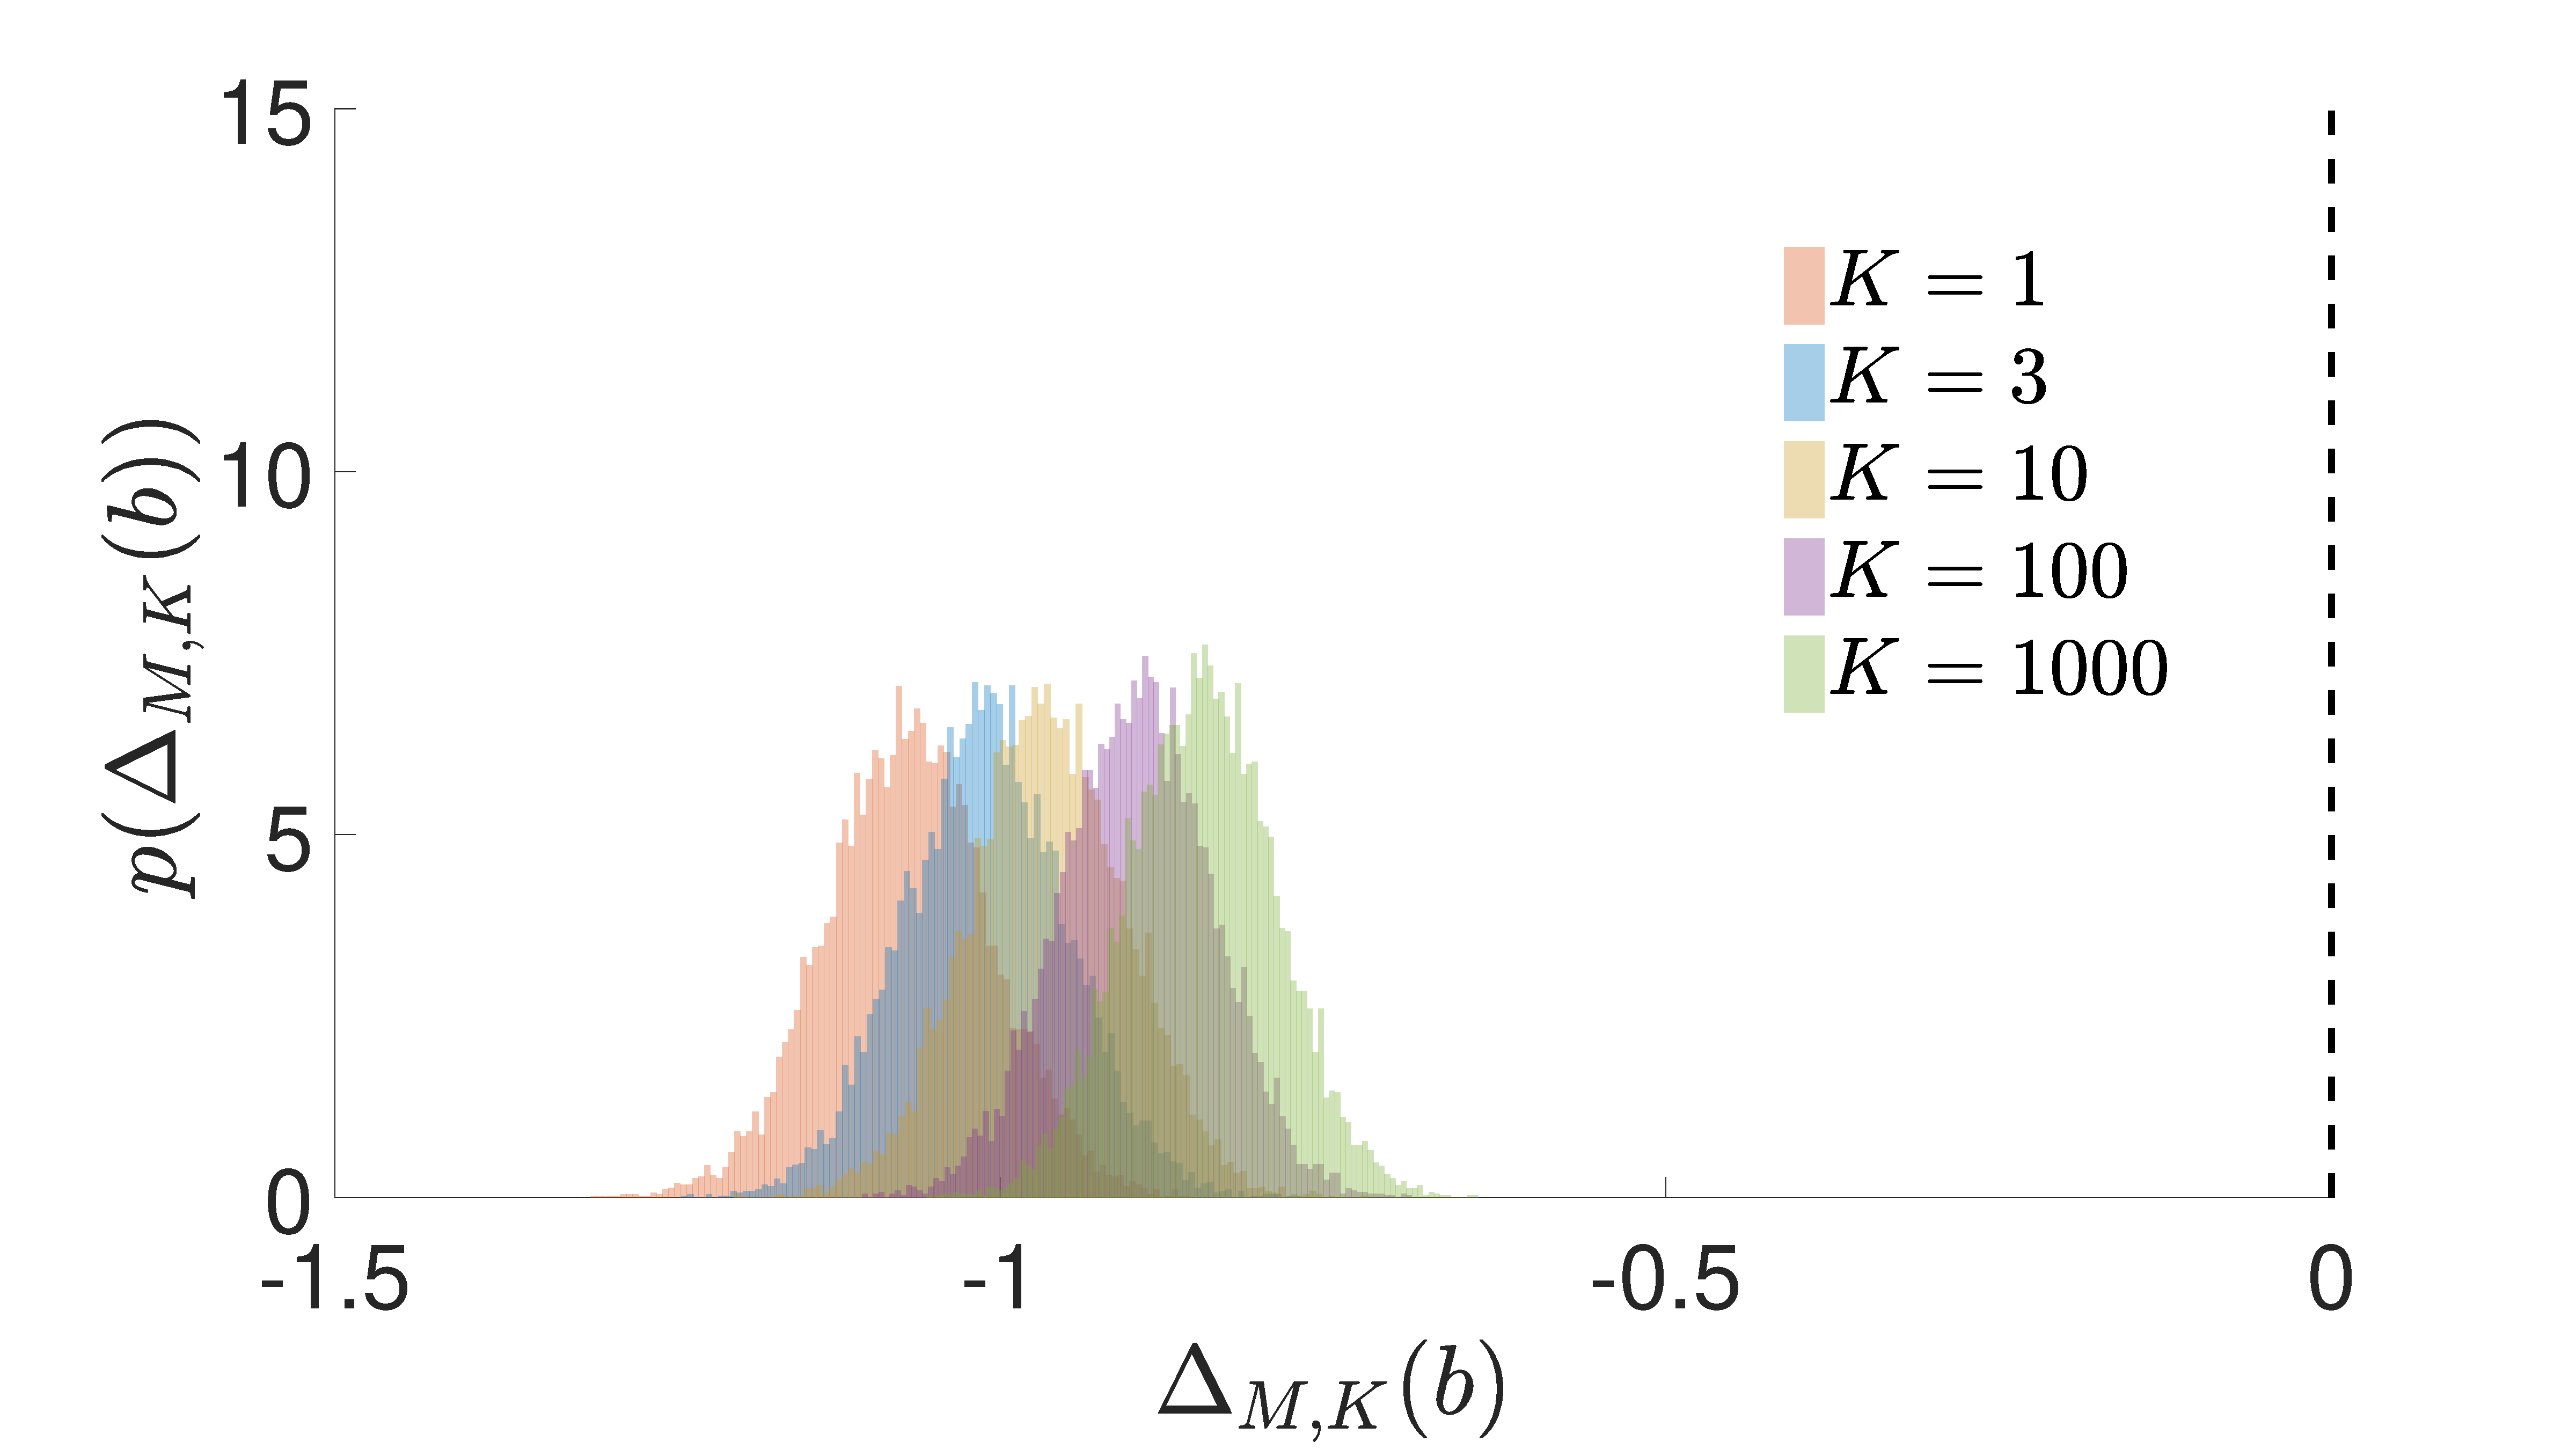
\includegraphics[width=\textwidth]{hv_b_hist_IWAE}
		\caption{\gls{IWAE} inference network gradient estimates \label{fig:hv/b_hist_iwae}}
	\end{subfigure} ~~~~~~~~~~
	\begin{subfigure}[b]{0.45\textwidth}
		\centering
		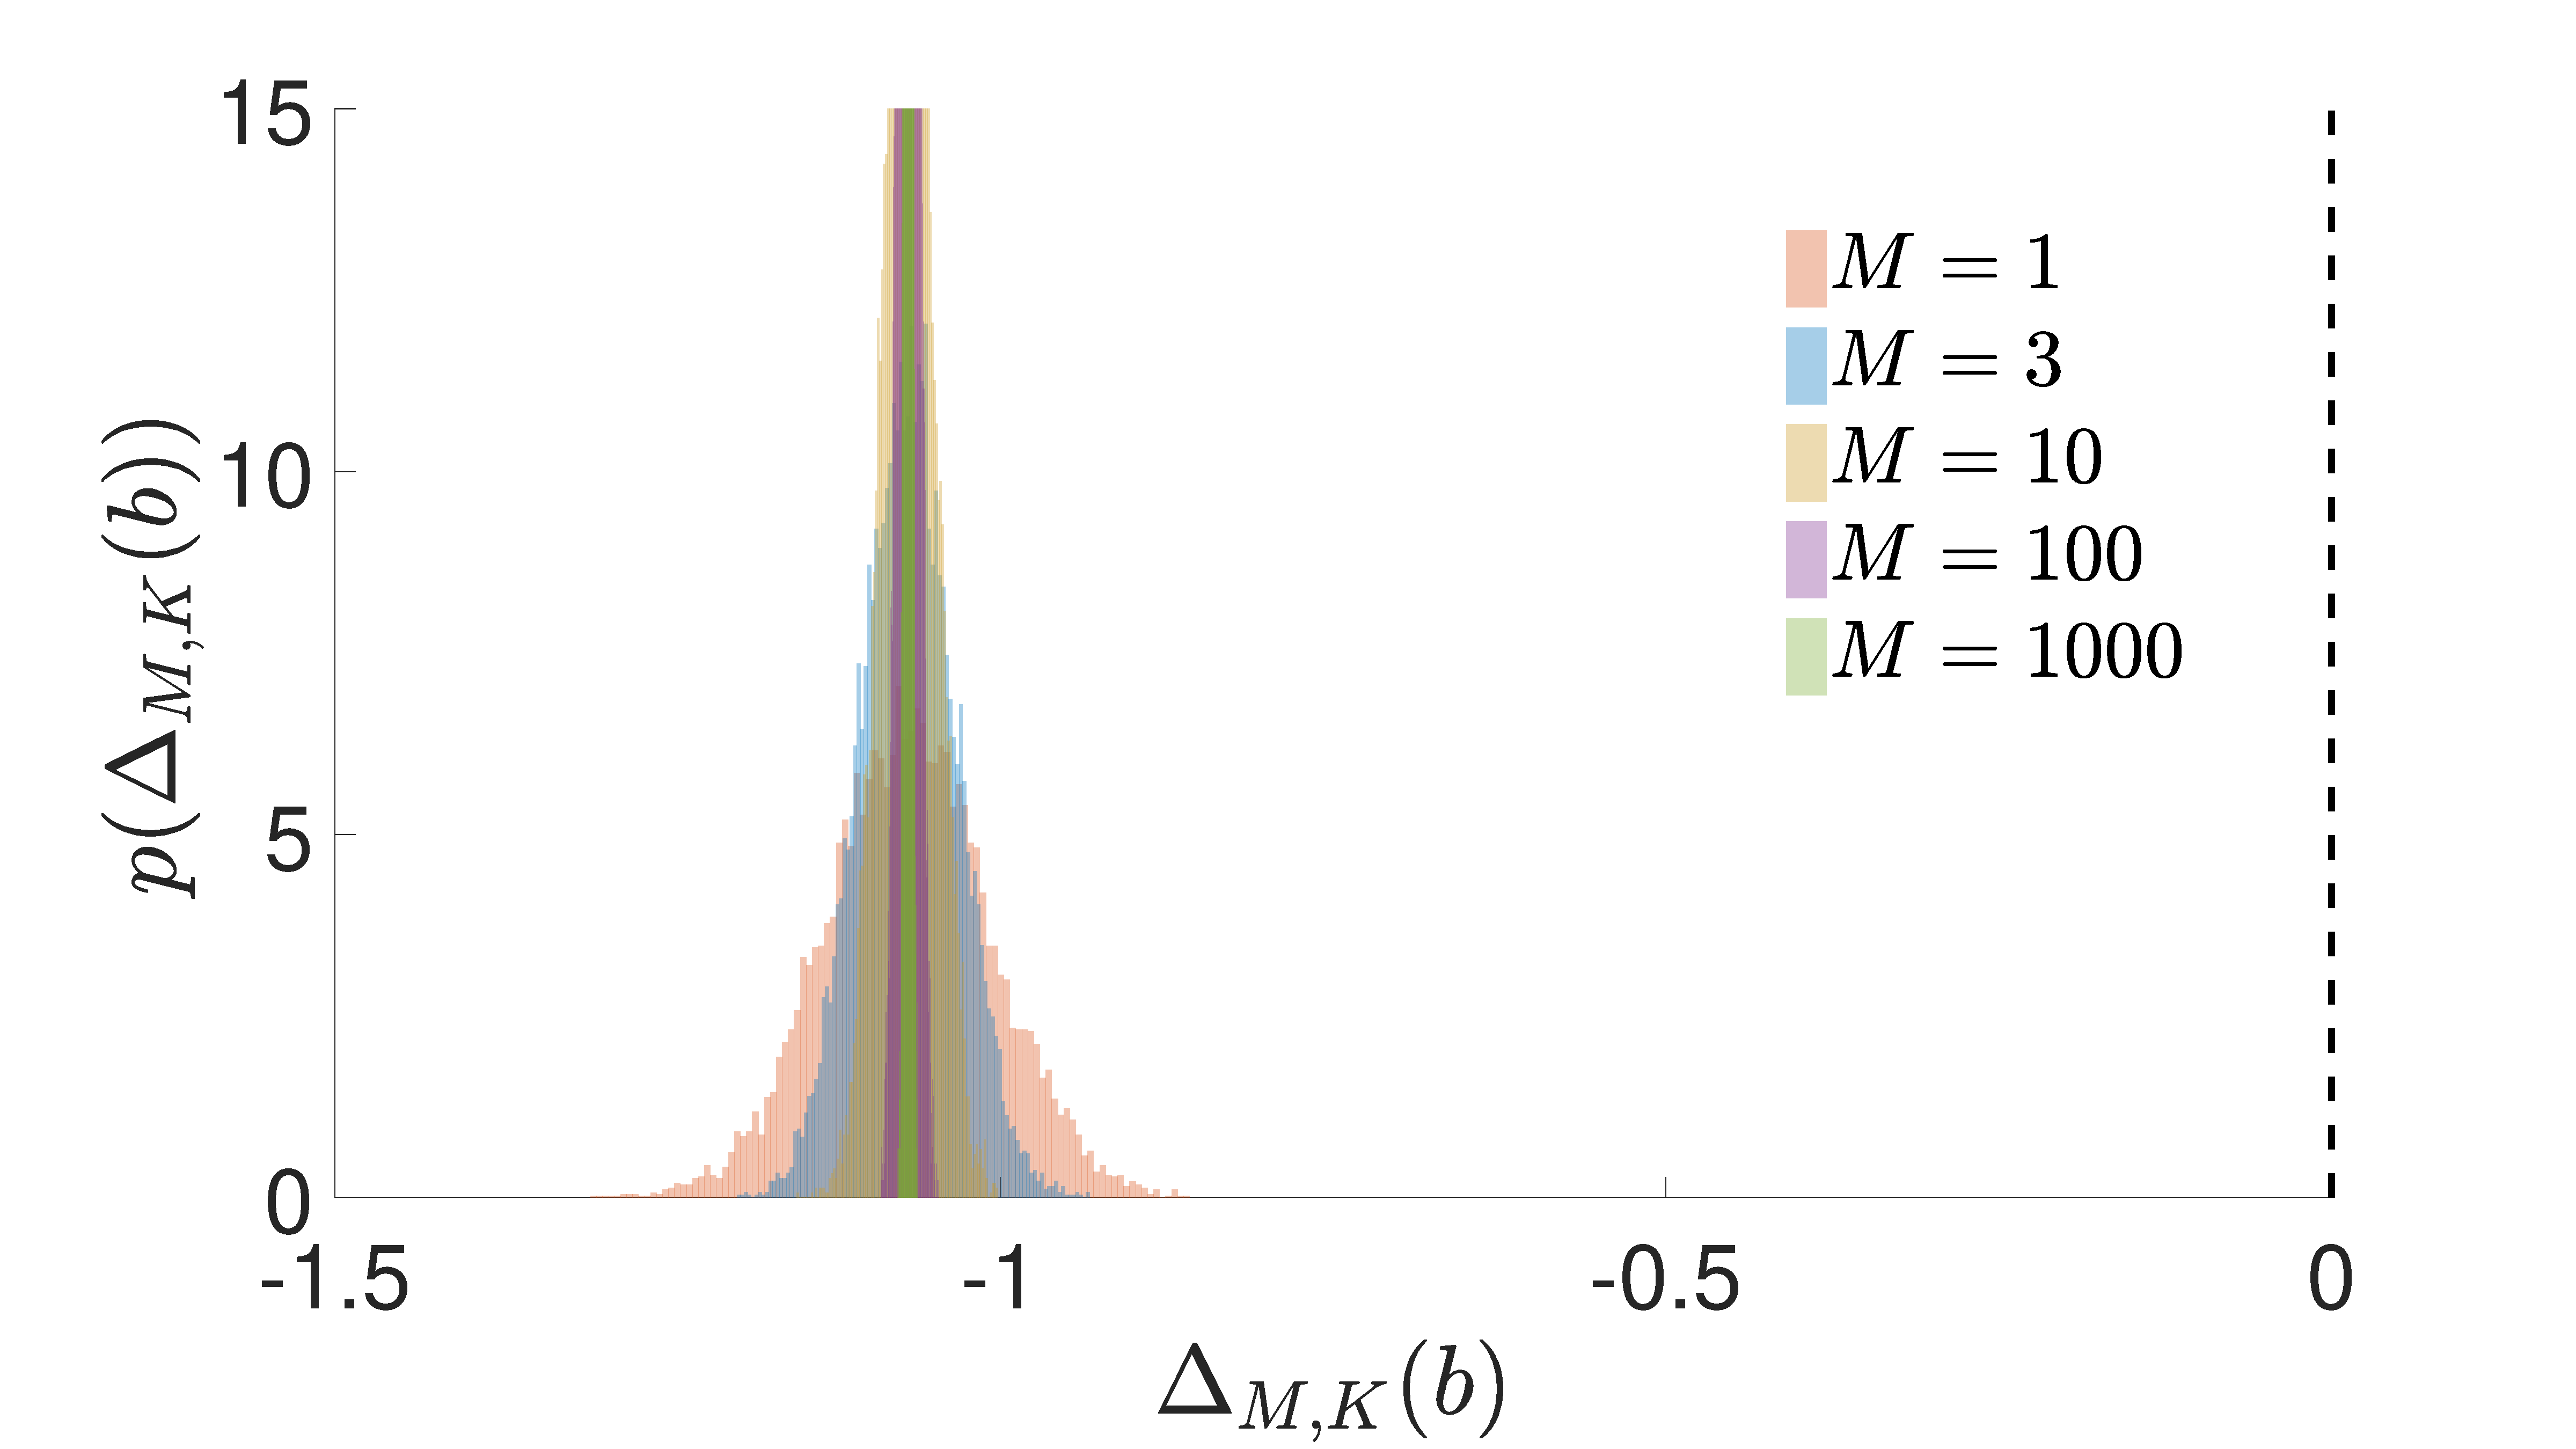
\includegraphics[width=\textwidth]{hv_b_hist_VAE}
		\caption{\gls{VAE} inference network gradient estimates \label{fig:hv/b_hist_vae}}
	\end{subfigure}\\
	\begin{subfigure}[b]{0.45\textwidth}
		\centering
		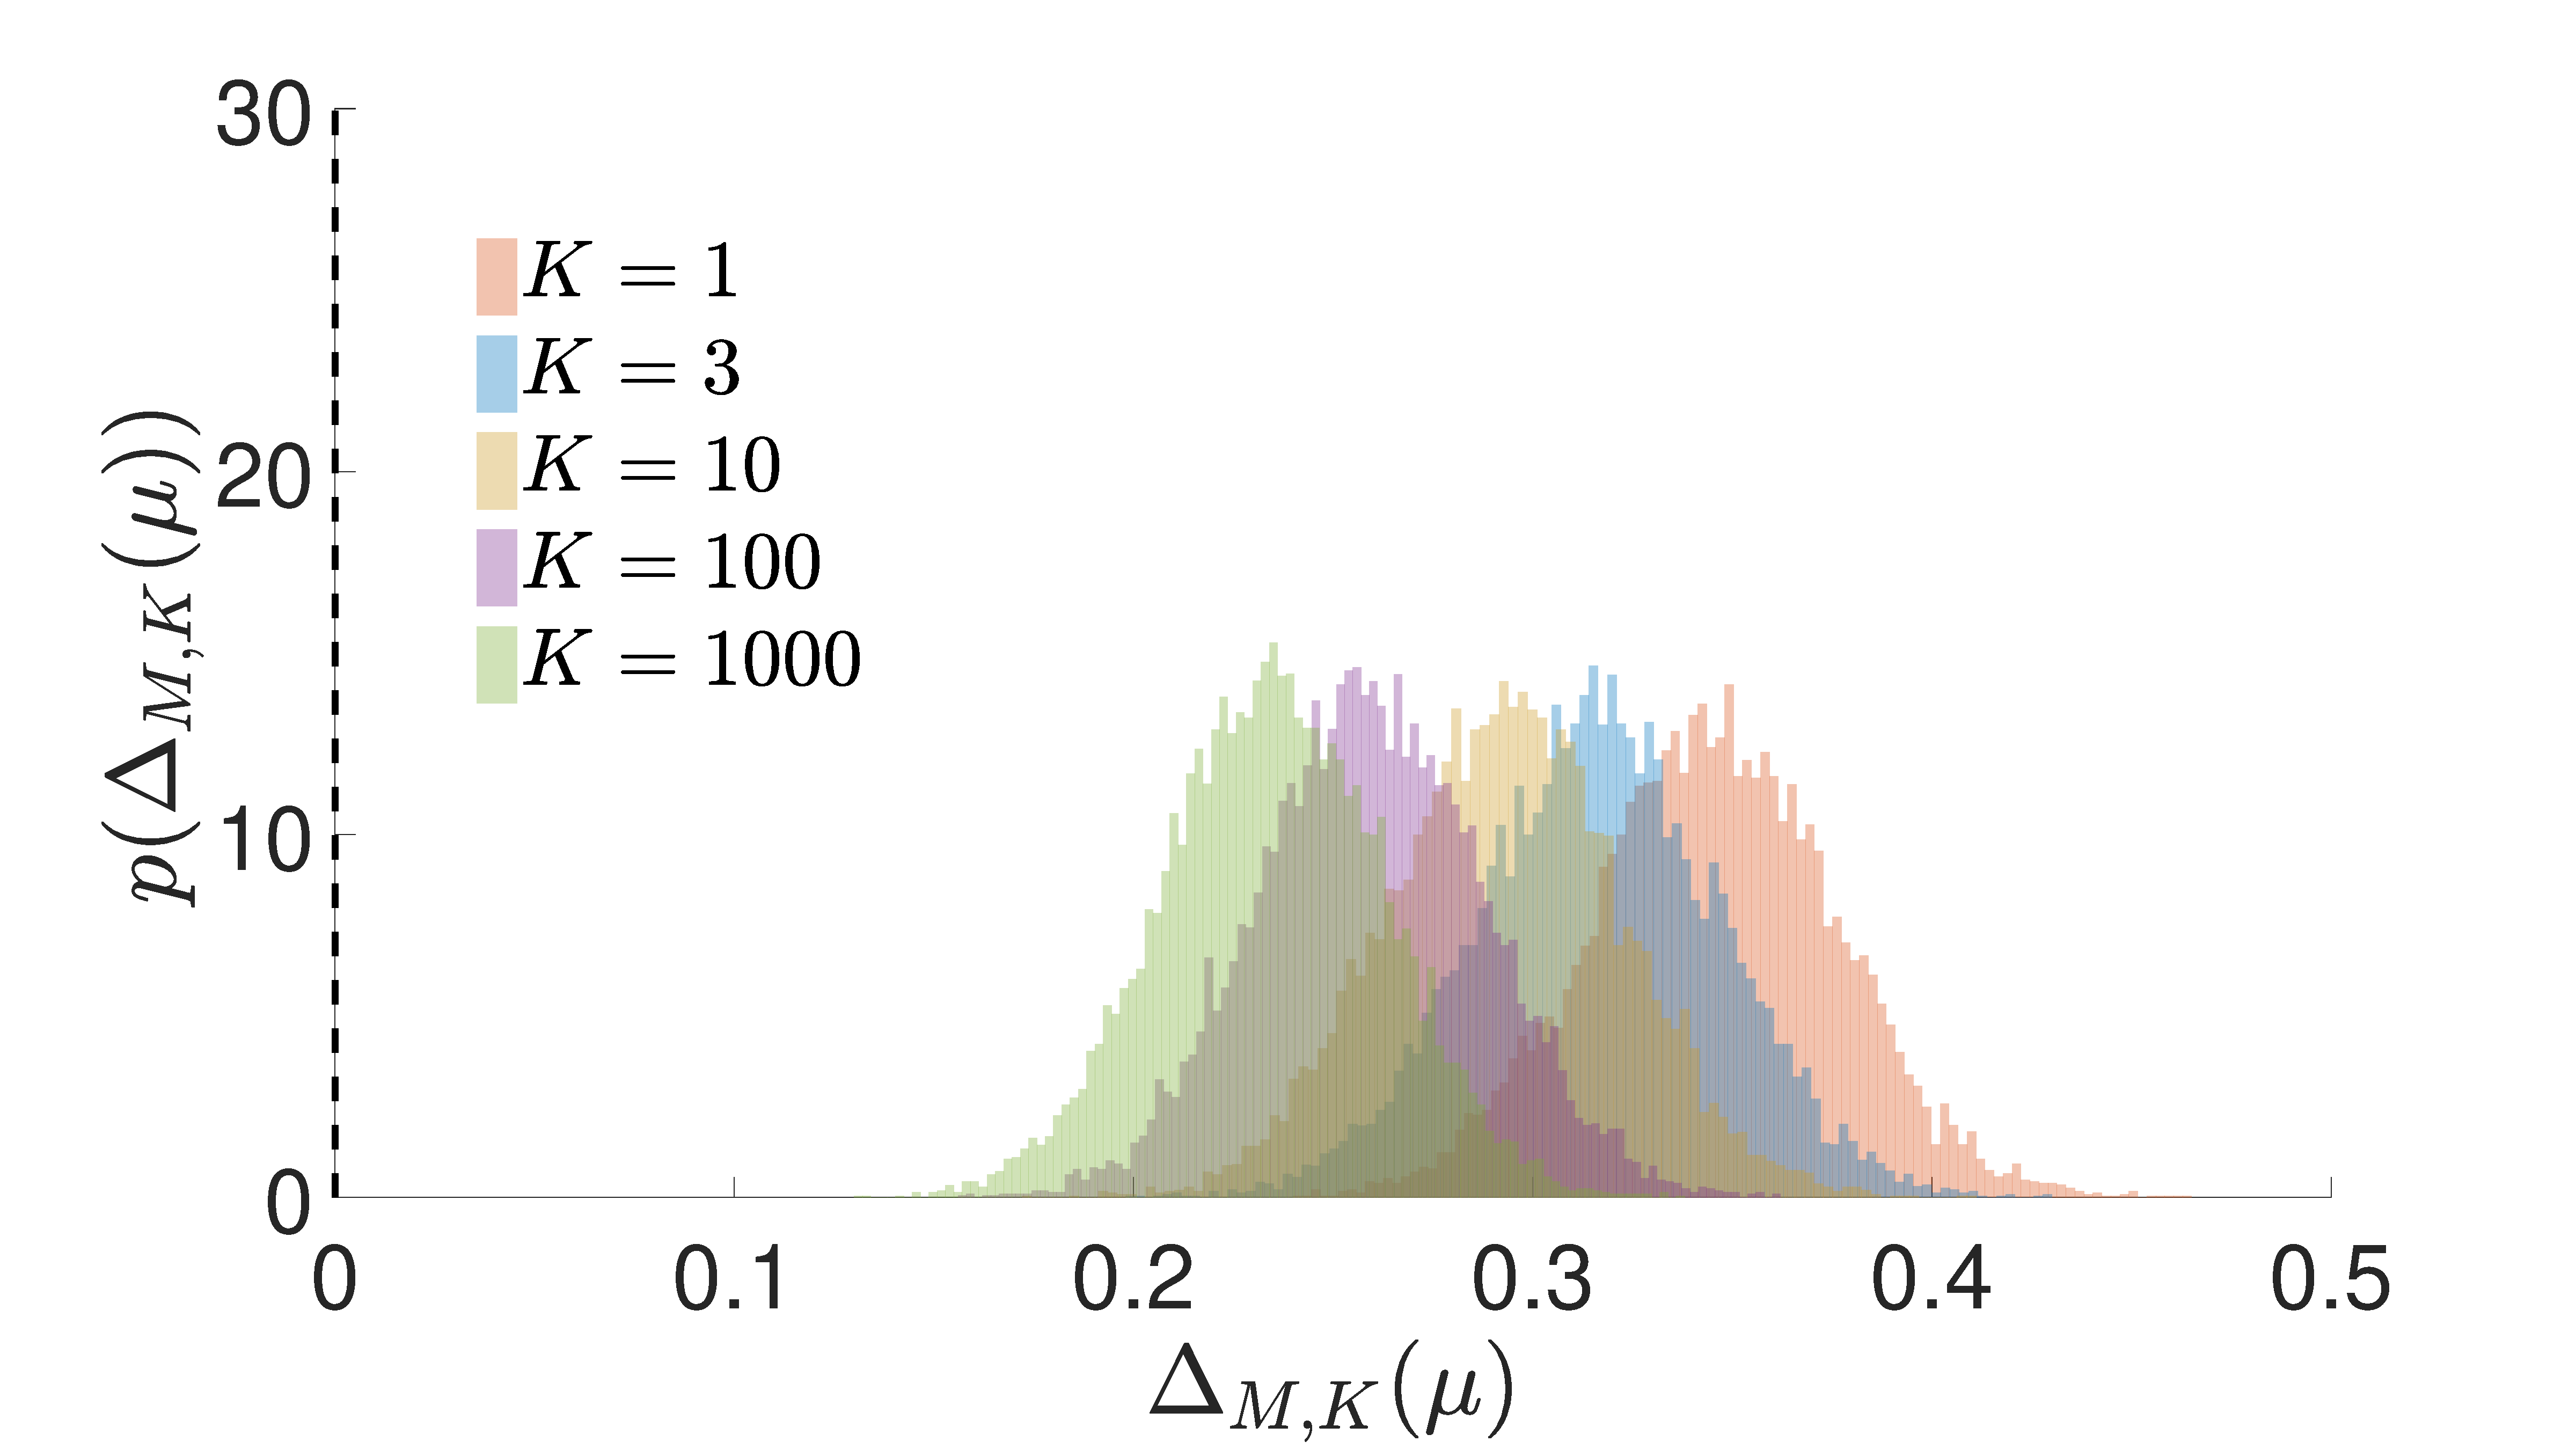
\includegraphics[width=\textwidth]{hv_mu_hist_IWAE}
		\caption{\gls{IWAE} generative network gradient estimates \label{fig:hv/mu_hist_iwae}}
	\end{subfigure} ~~~~~~~~~~
	\begin{subfigure}[b]{0.45\textwidth}
		\centering
		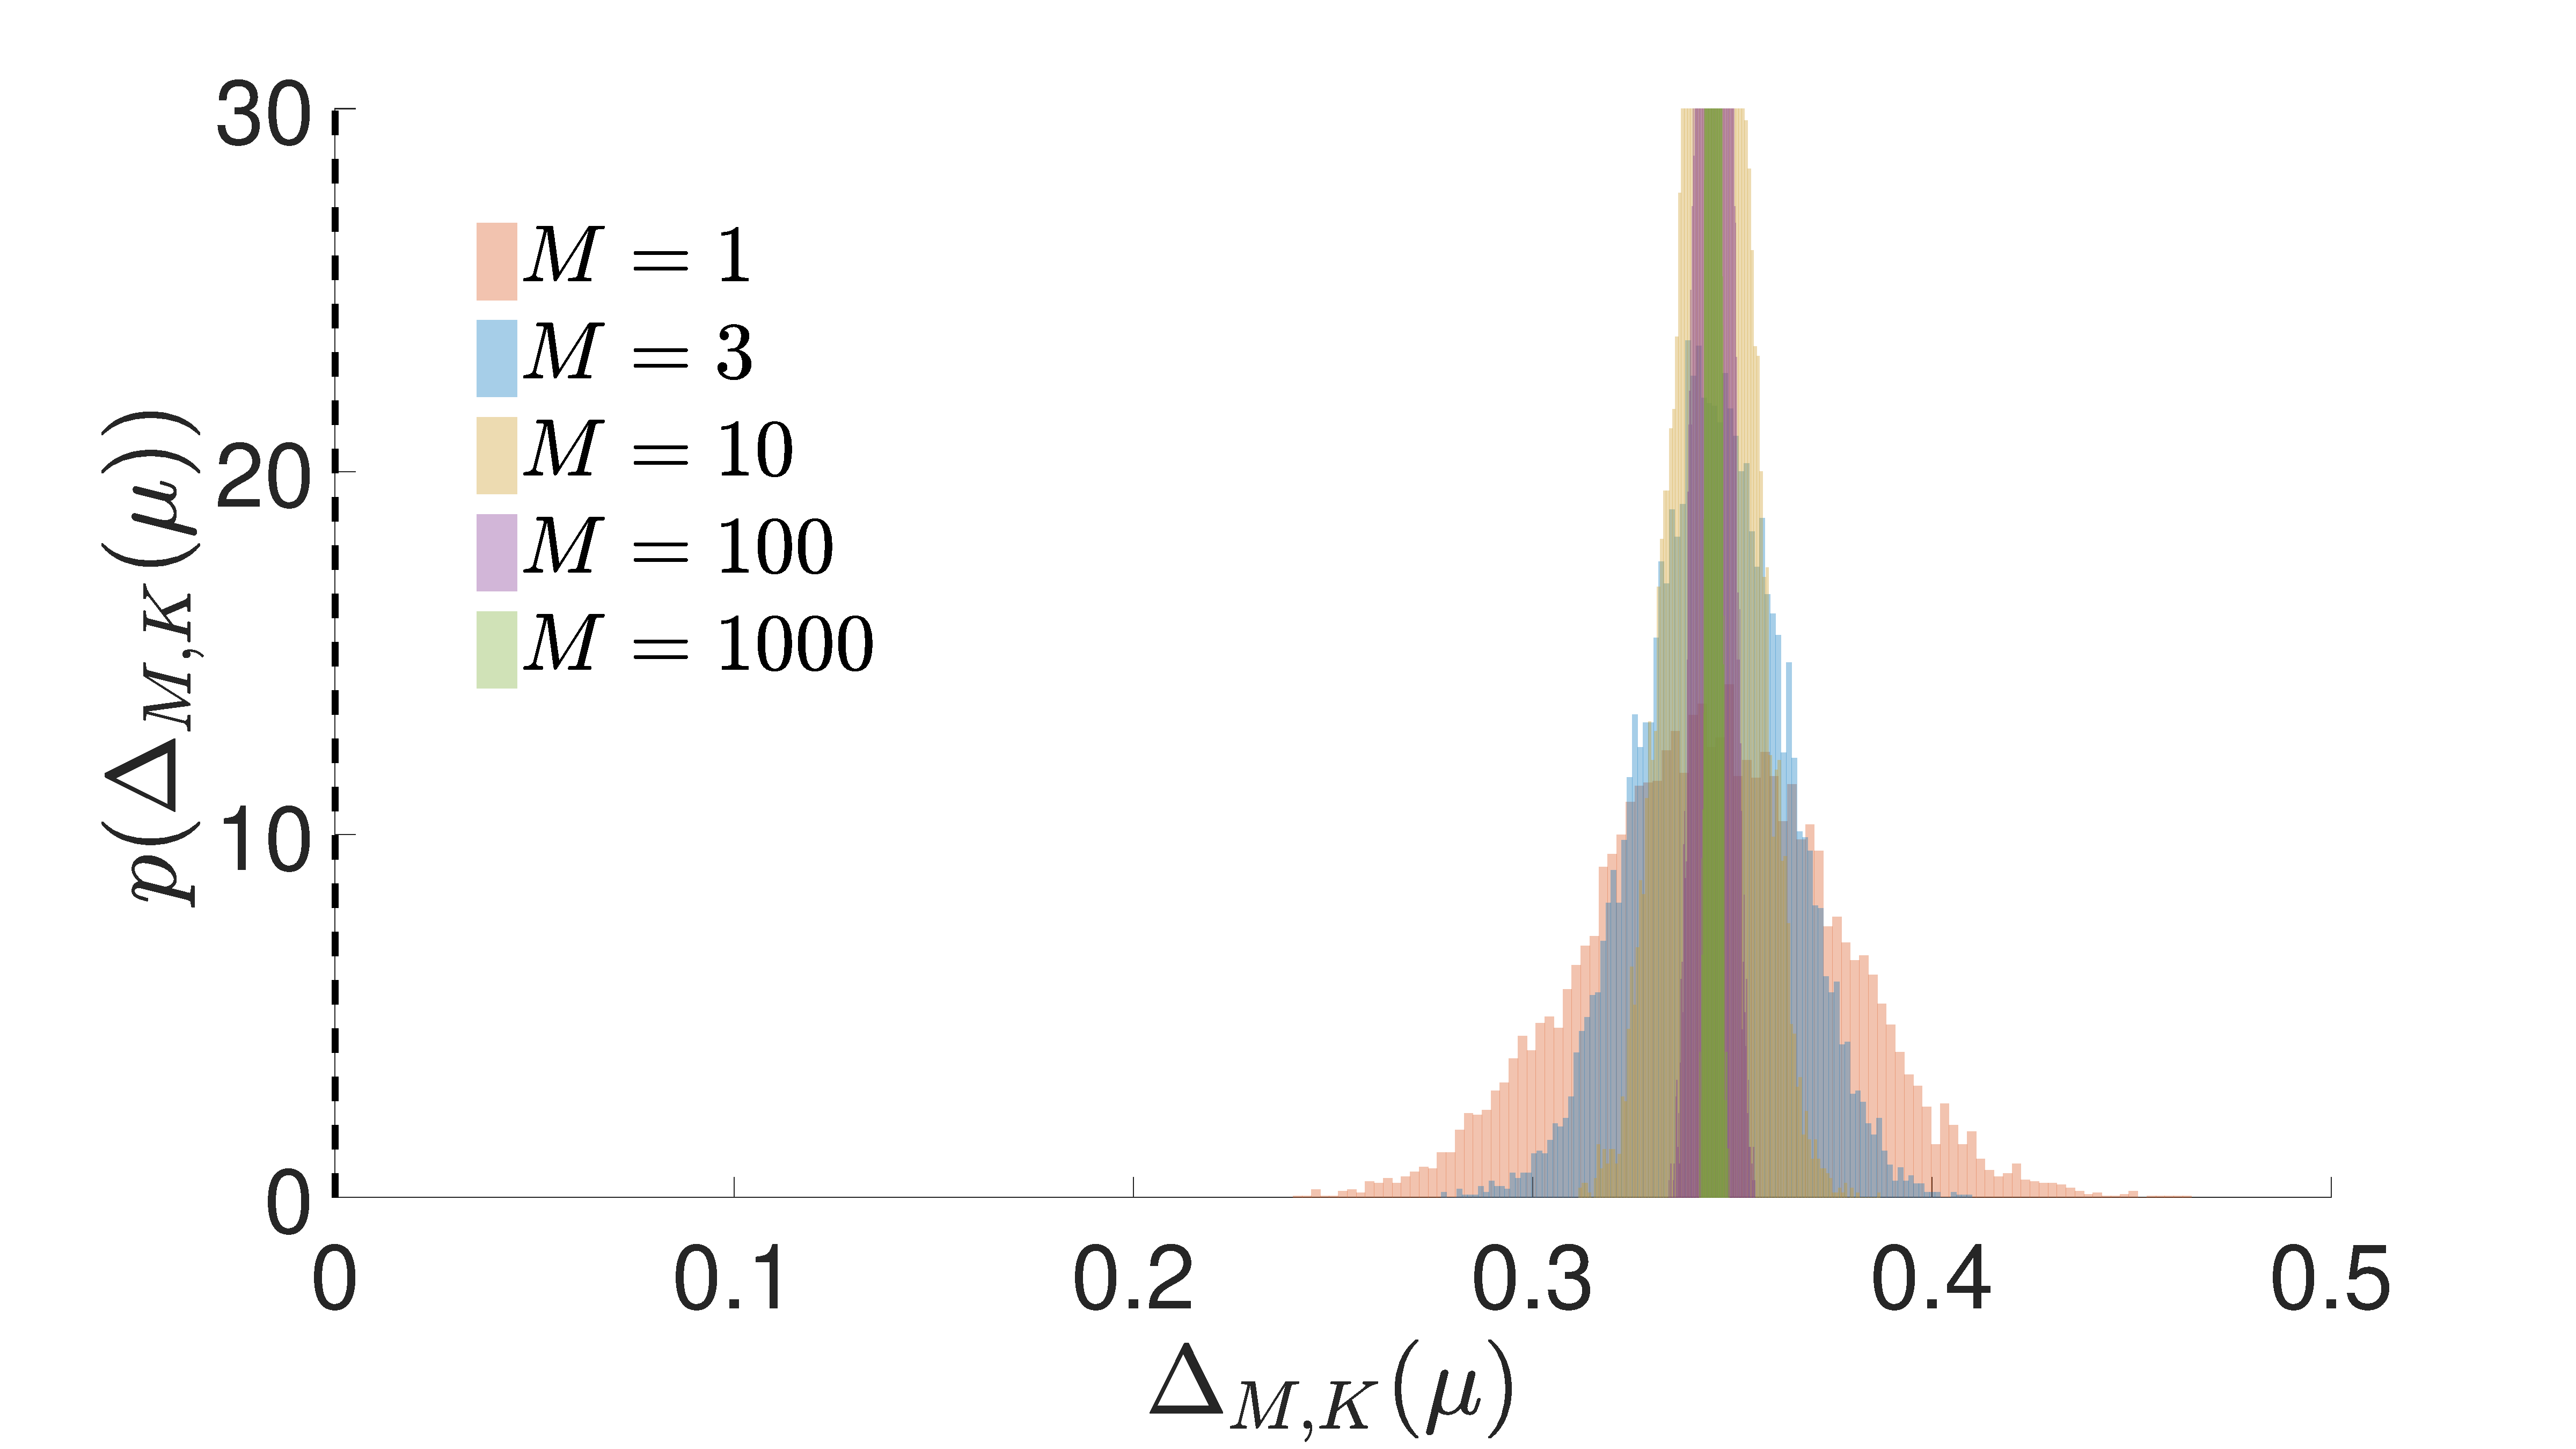
\includegraphics[width=\textwidth]{hv_mu_hist_VAE}
		\caption{\gls{VAE} generative network gradient estimates \label{fig:hv/mu_hist_vae}}
	\end{subfigure}
	\caption{Histograms of gradient estimates as per Figure~\ref{fig:snr/hists}.
		\label{fig:hv/hists}
	\vspace{-4pt}}
\end{figure}

\begin{figure}[h]
	\centering
	\begin{subfigure}[b]{0.45\textwidth}
		\centering
		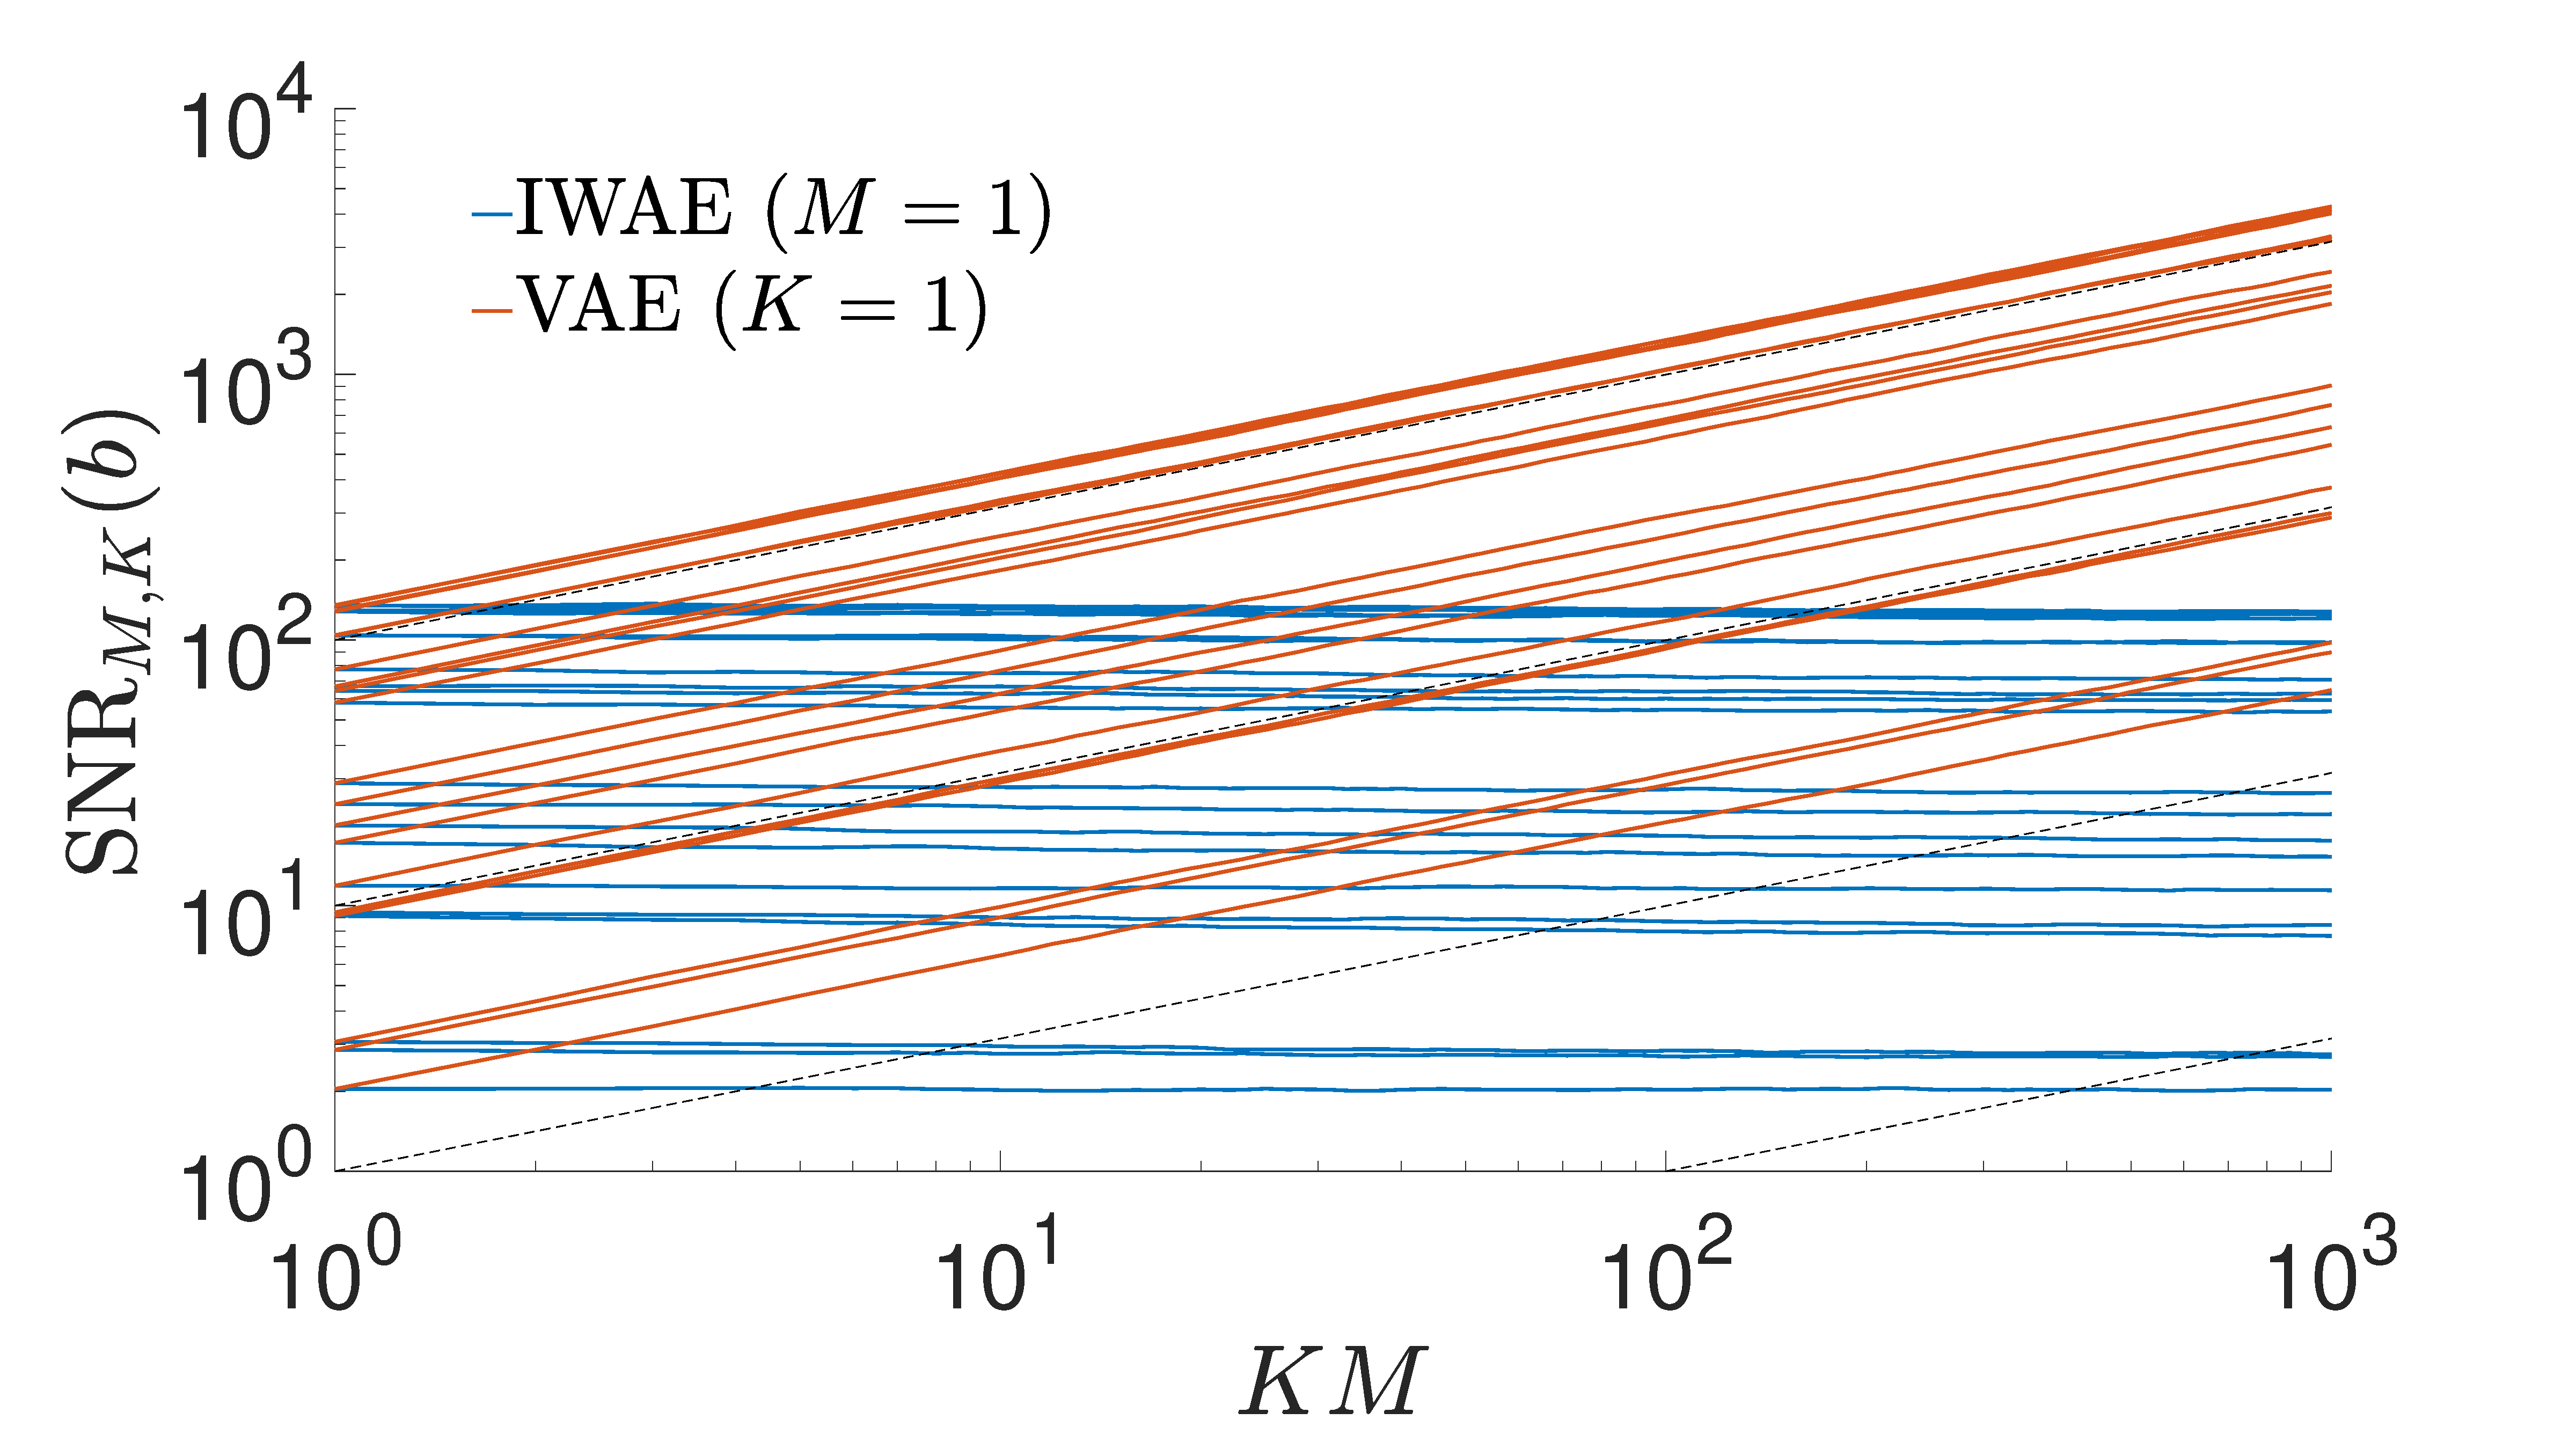
\includegraphics[width=\textwidth]{hv_b_conv}
		\caption{Convergence of \gls{SNR} for inference network \label{fig:hv/b}}
	\end{subfigure} ~~~~~~~~~~
	\begin{subfigure}[b]{0.45\textwidth}
		\centering
		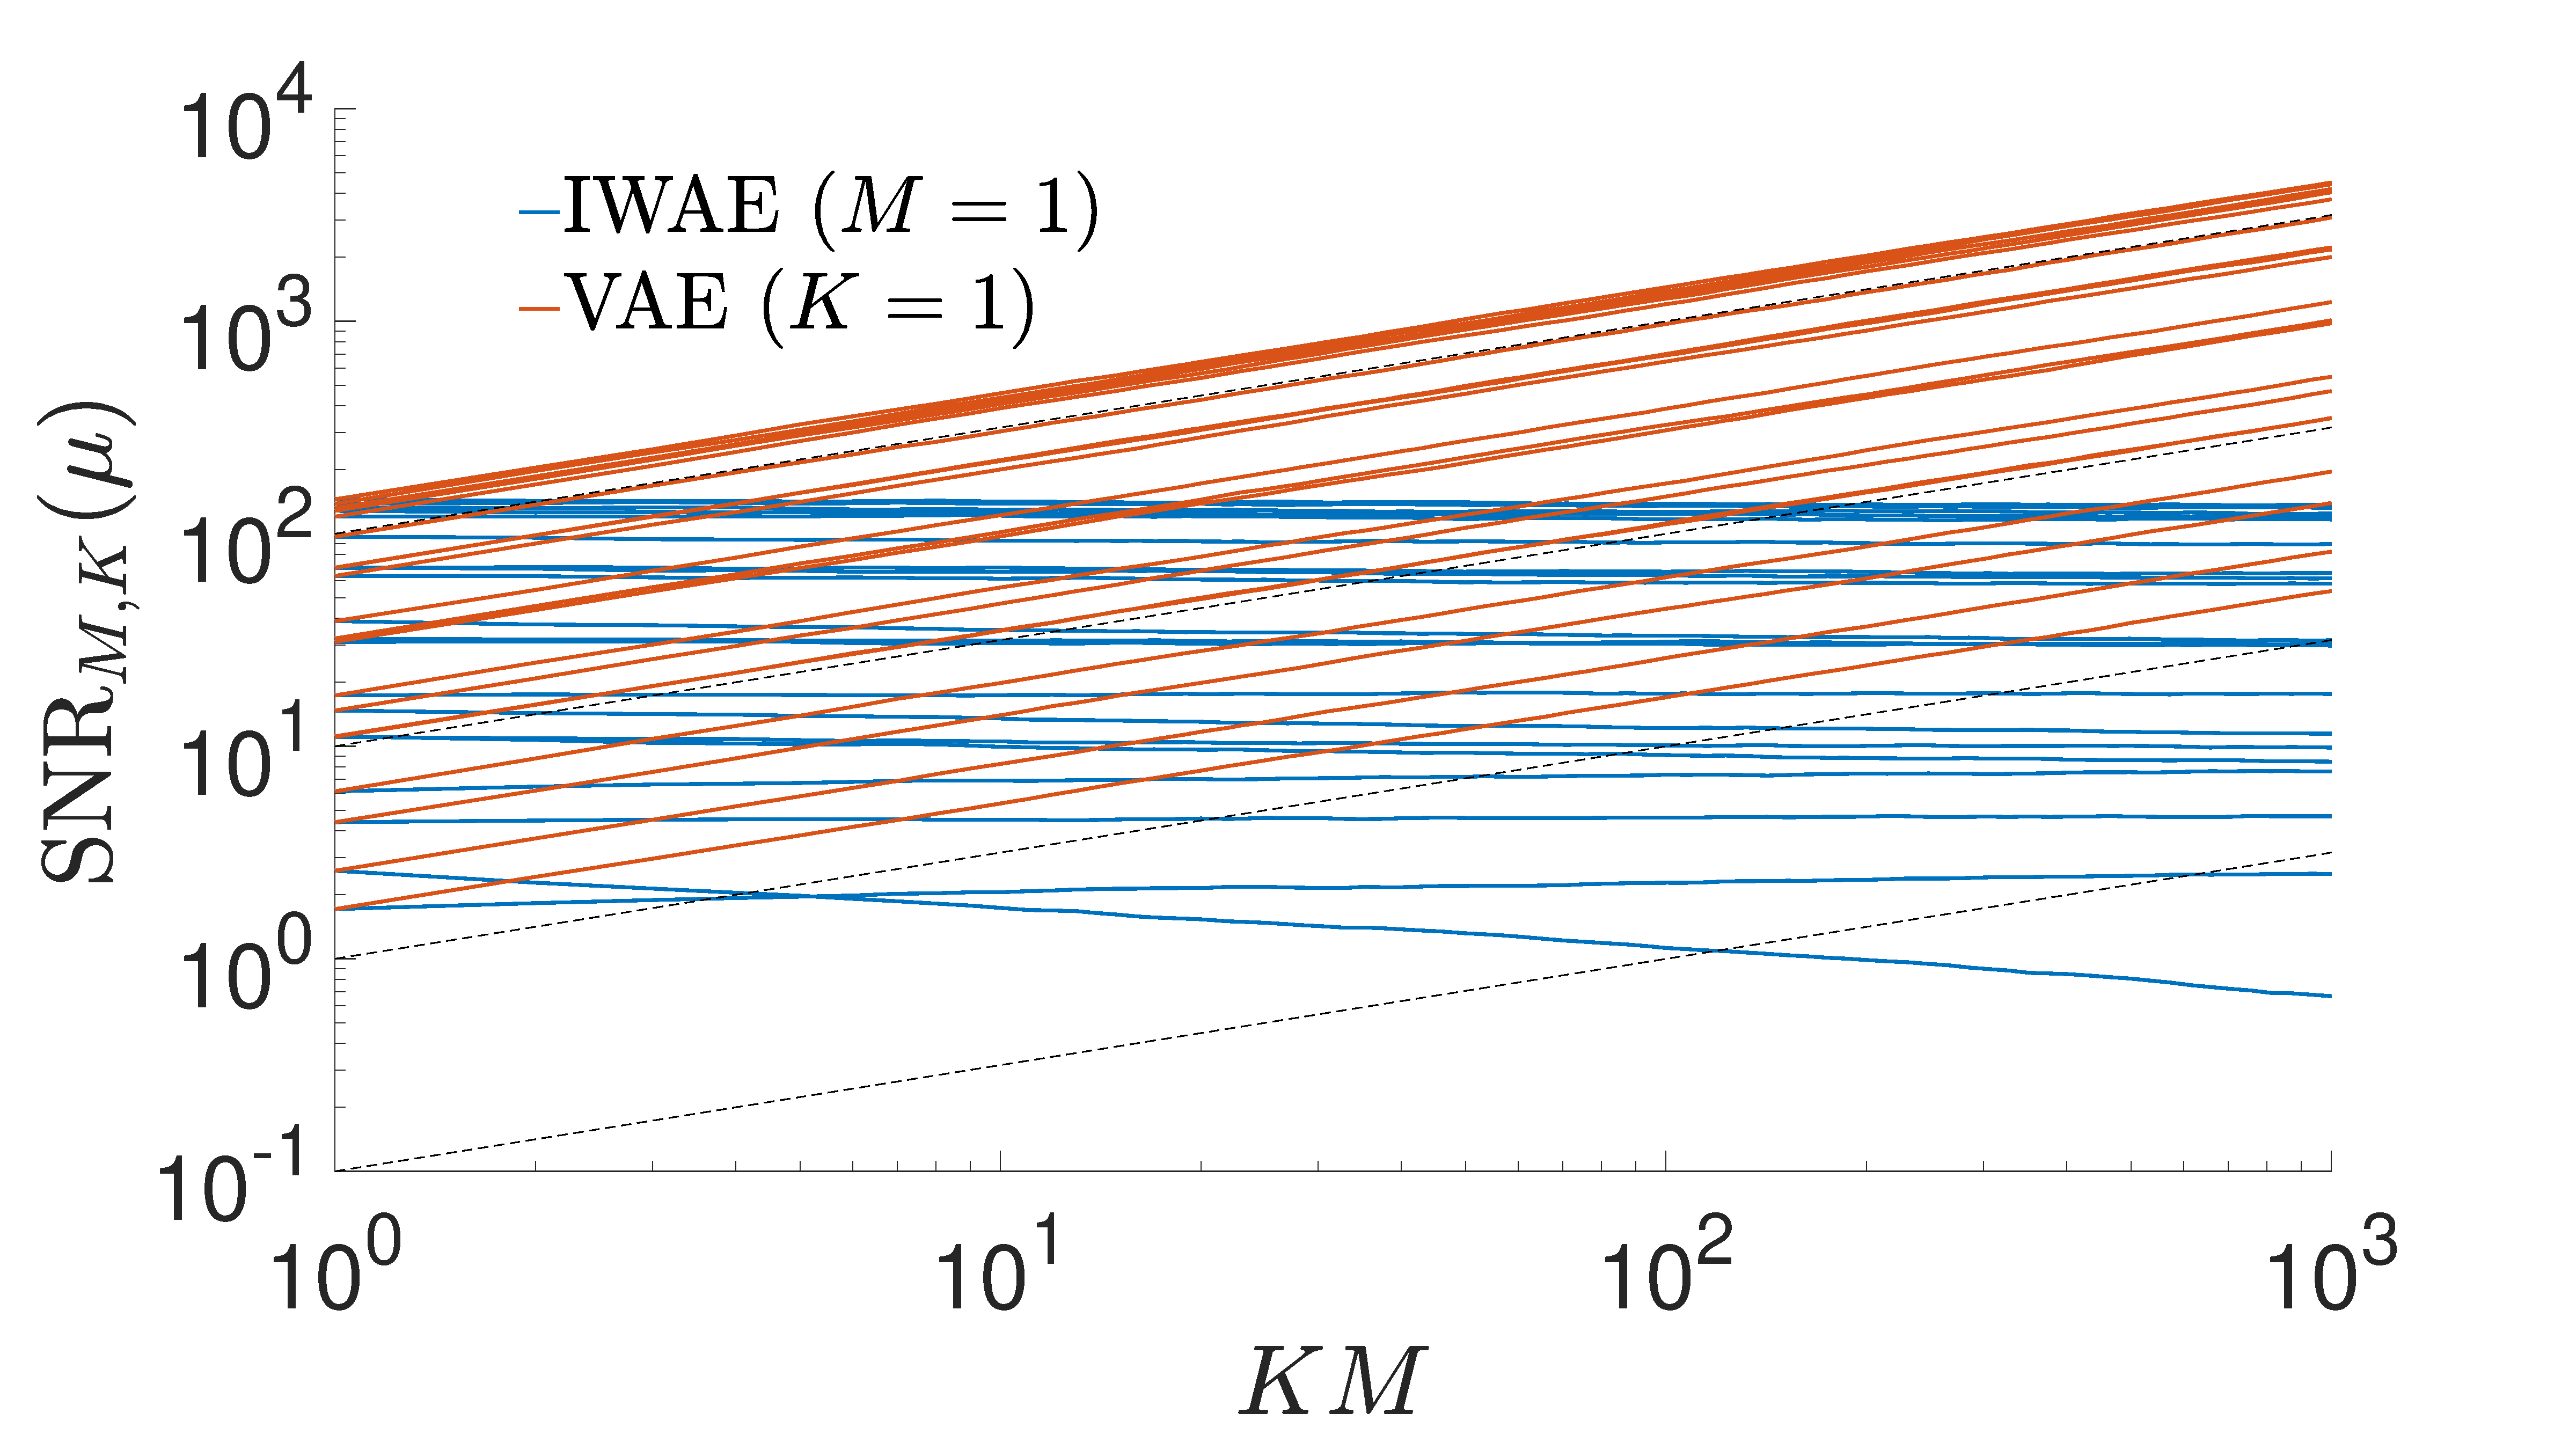
\includegraphics[width=\textwidth]{hv_mu_conv}
		\caption{Convergence of \gls{SNR} for generative network\label{fig:hv/mu}}
	\end{subfigure}
	\caption{Convergence of signal-to-noise ratios of gradient estimates
		as per Figure~\ref{fig:snr/K_conv}.
		\label{fig:hv/K_conv}}
\end{figure}


\begin{figure}[h]
	\centering
	\begin{subfigure}[b]{0.45\textwidth}
		\centering
		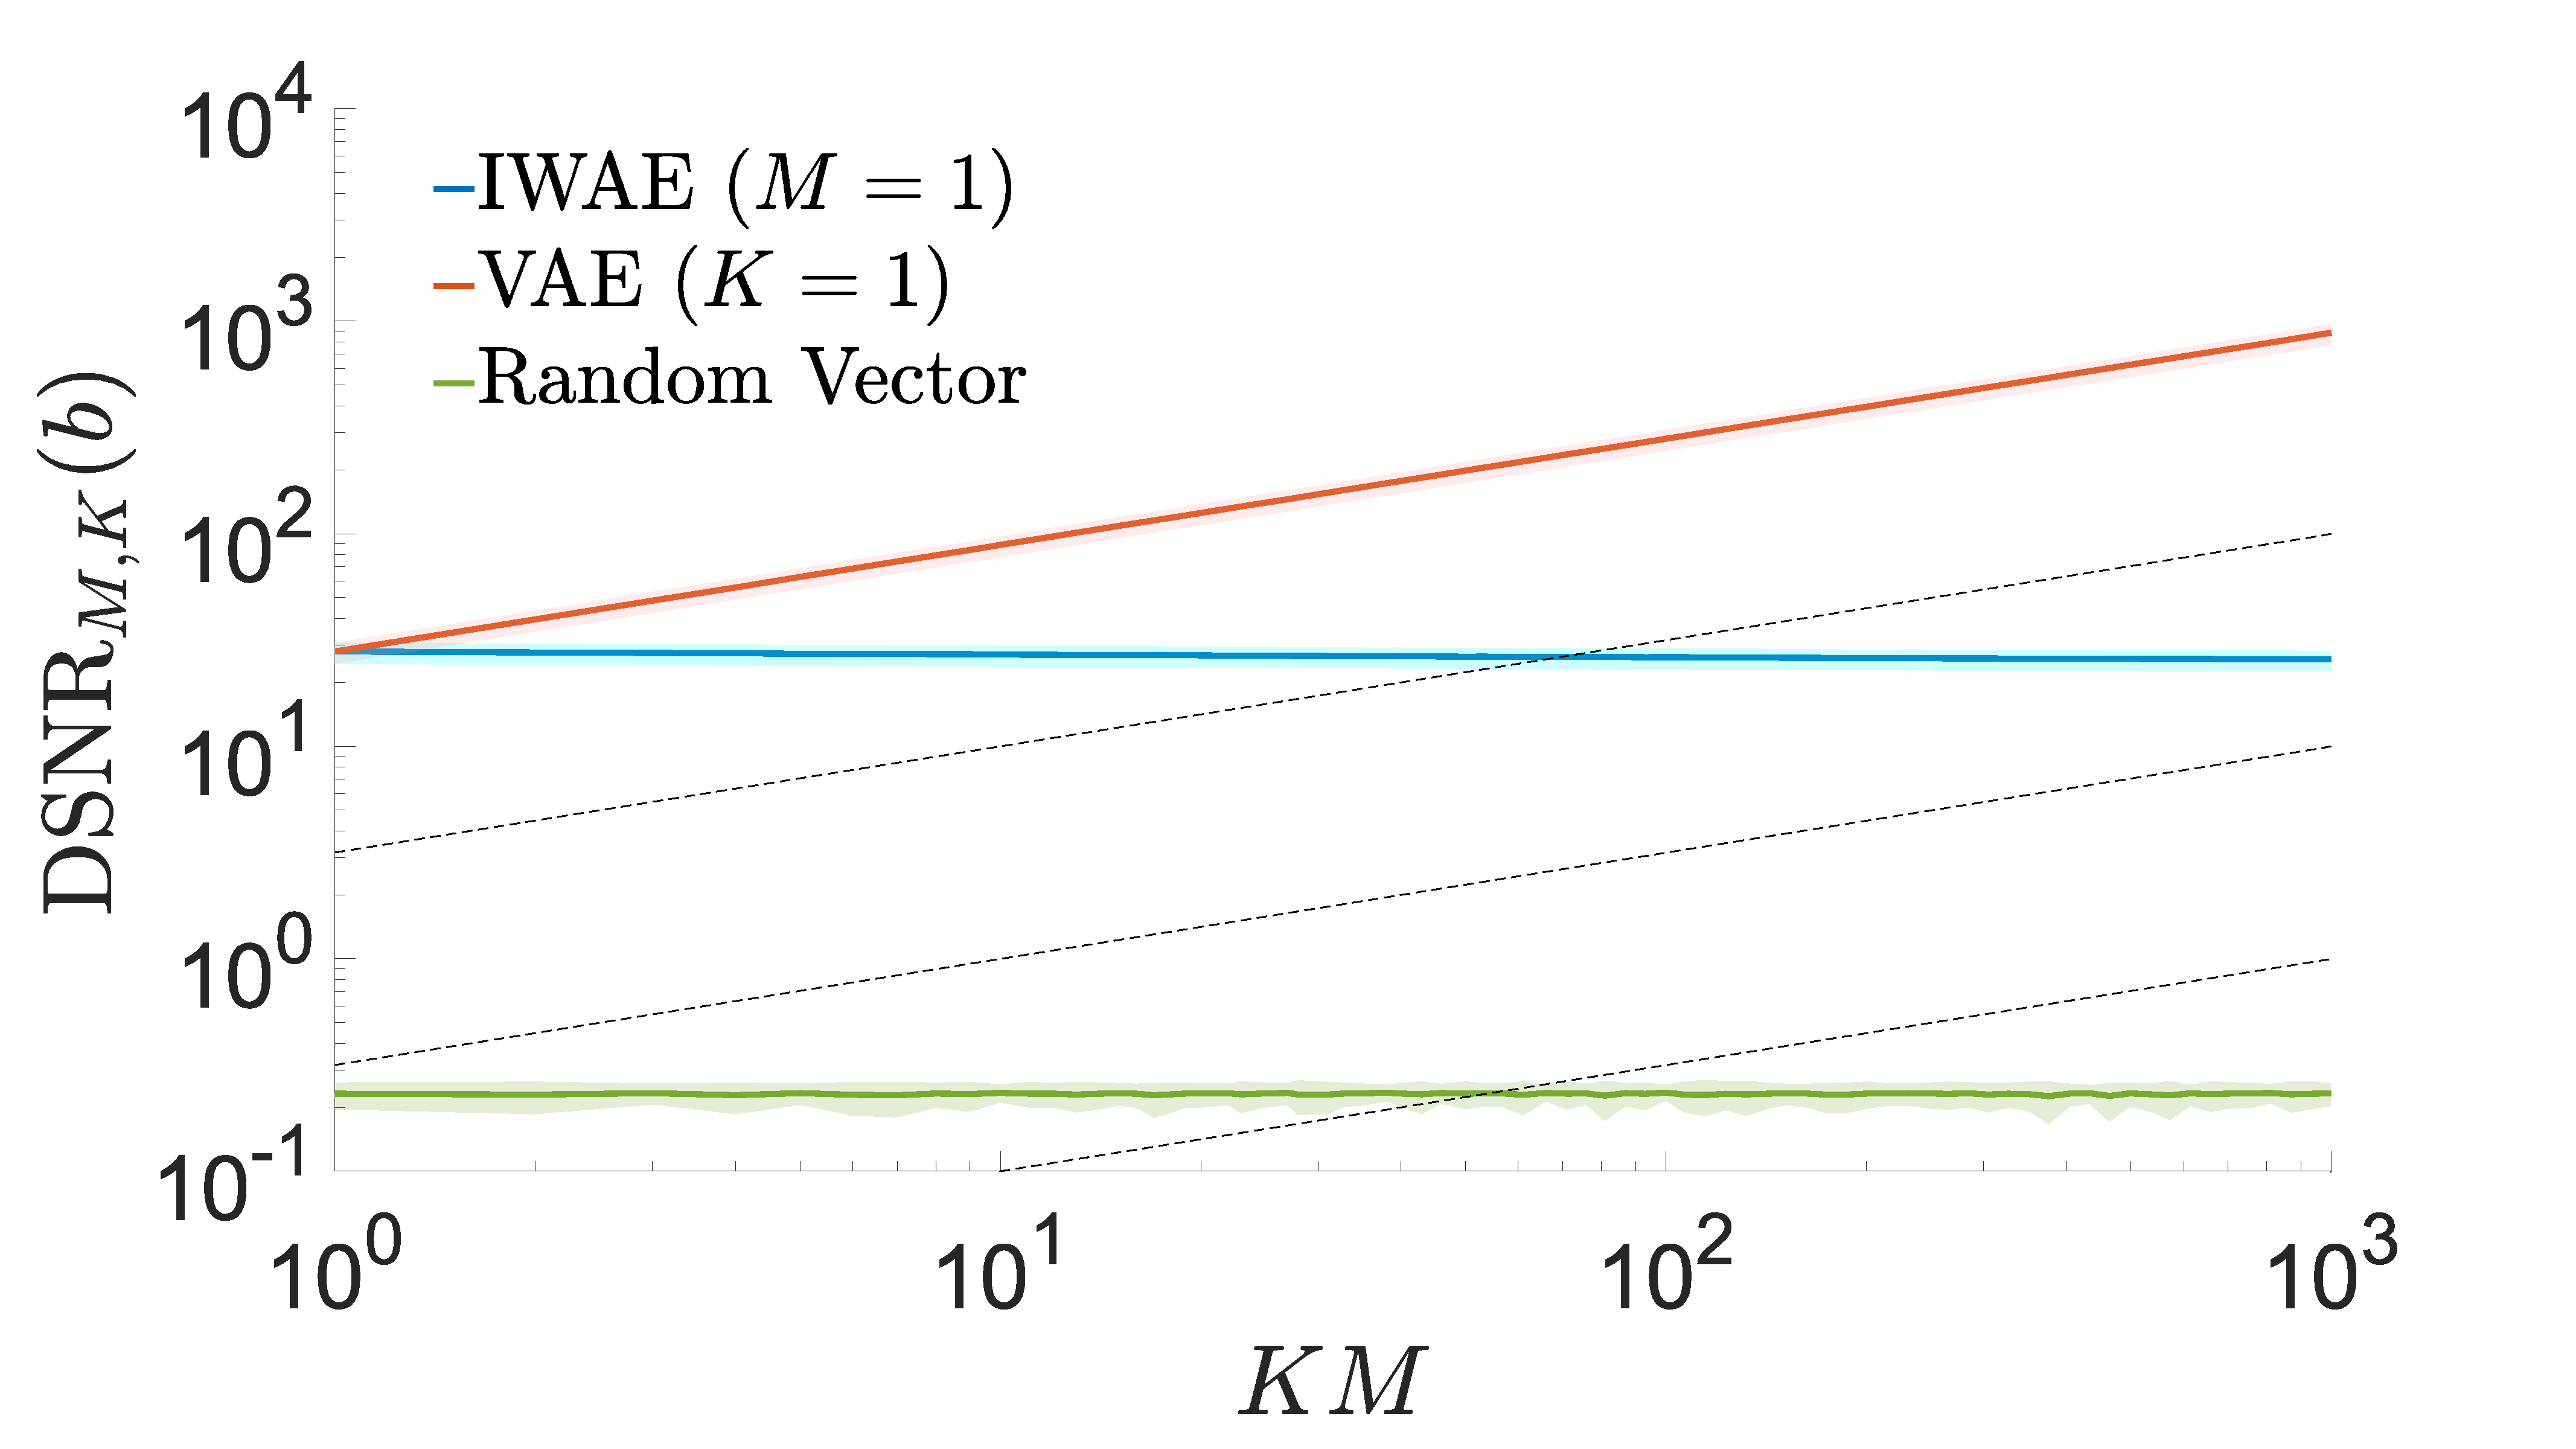
\includegraphics[width=\textwidth]{hv_snr_dir}
		\caption{Convergence of \textsc{dsnr} for inference network\label{fig:hv/snr_dir}}
	\end{subfigure}~~~~~~~~~~
	\begin{subfigure}[b]{0.45\textwidth}
		\centering
		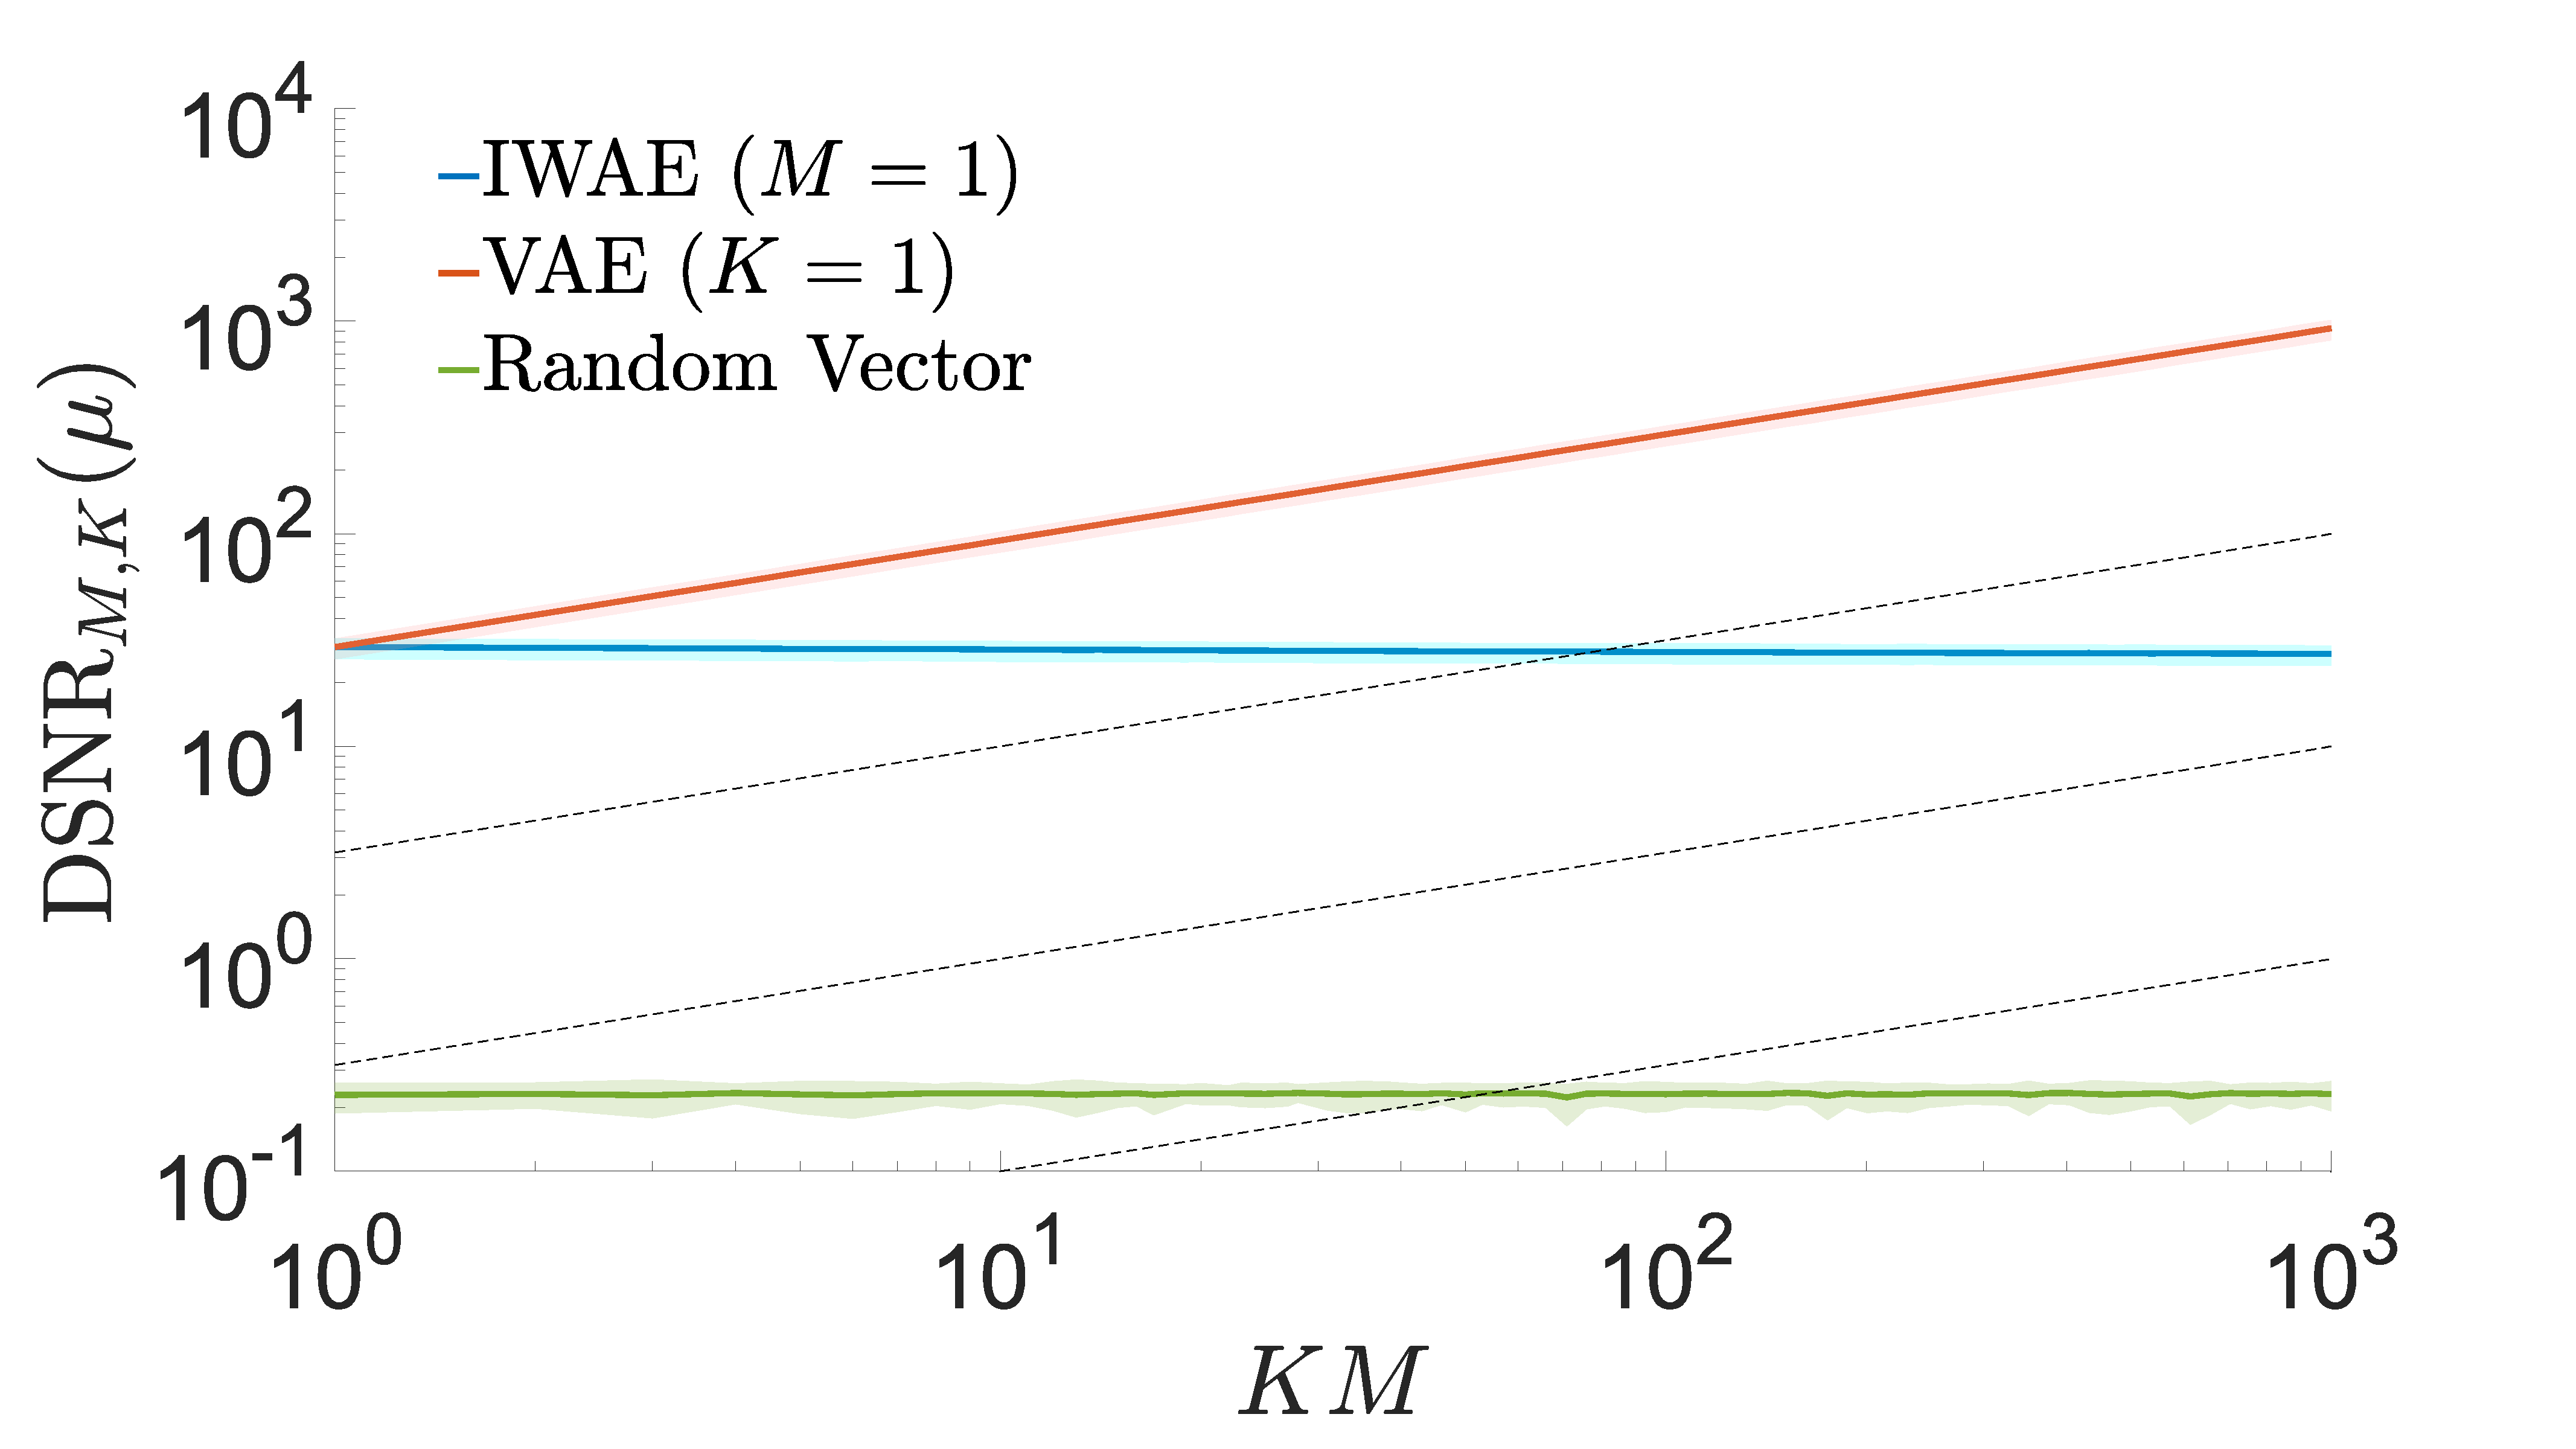
\includegraphics[width=\textwidth]{hv_snr_dir_mu}
		\caption{Convergence of \textsc{dsnr} for generative network\label{fig:hv/snr_dir_mu}}
	\end{subfigure}
	\caption{Convergence of directional signal-to-noise ratio of gradients estimates 
		as per Figure~\ref{fig:snr/extra}.
		\label{fig:hv/extra_end}}
\end{figure}

\begin{figure}[h]
	\centering
	\begin{subfigure}[b]{0.45\textwidth}
		\centering
		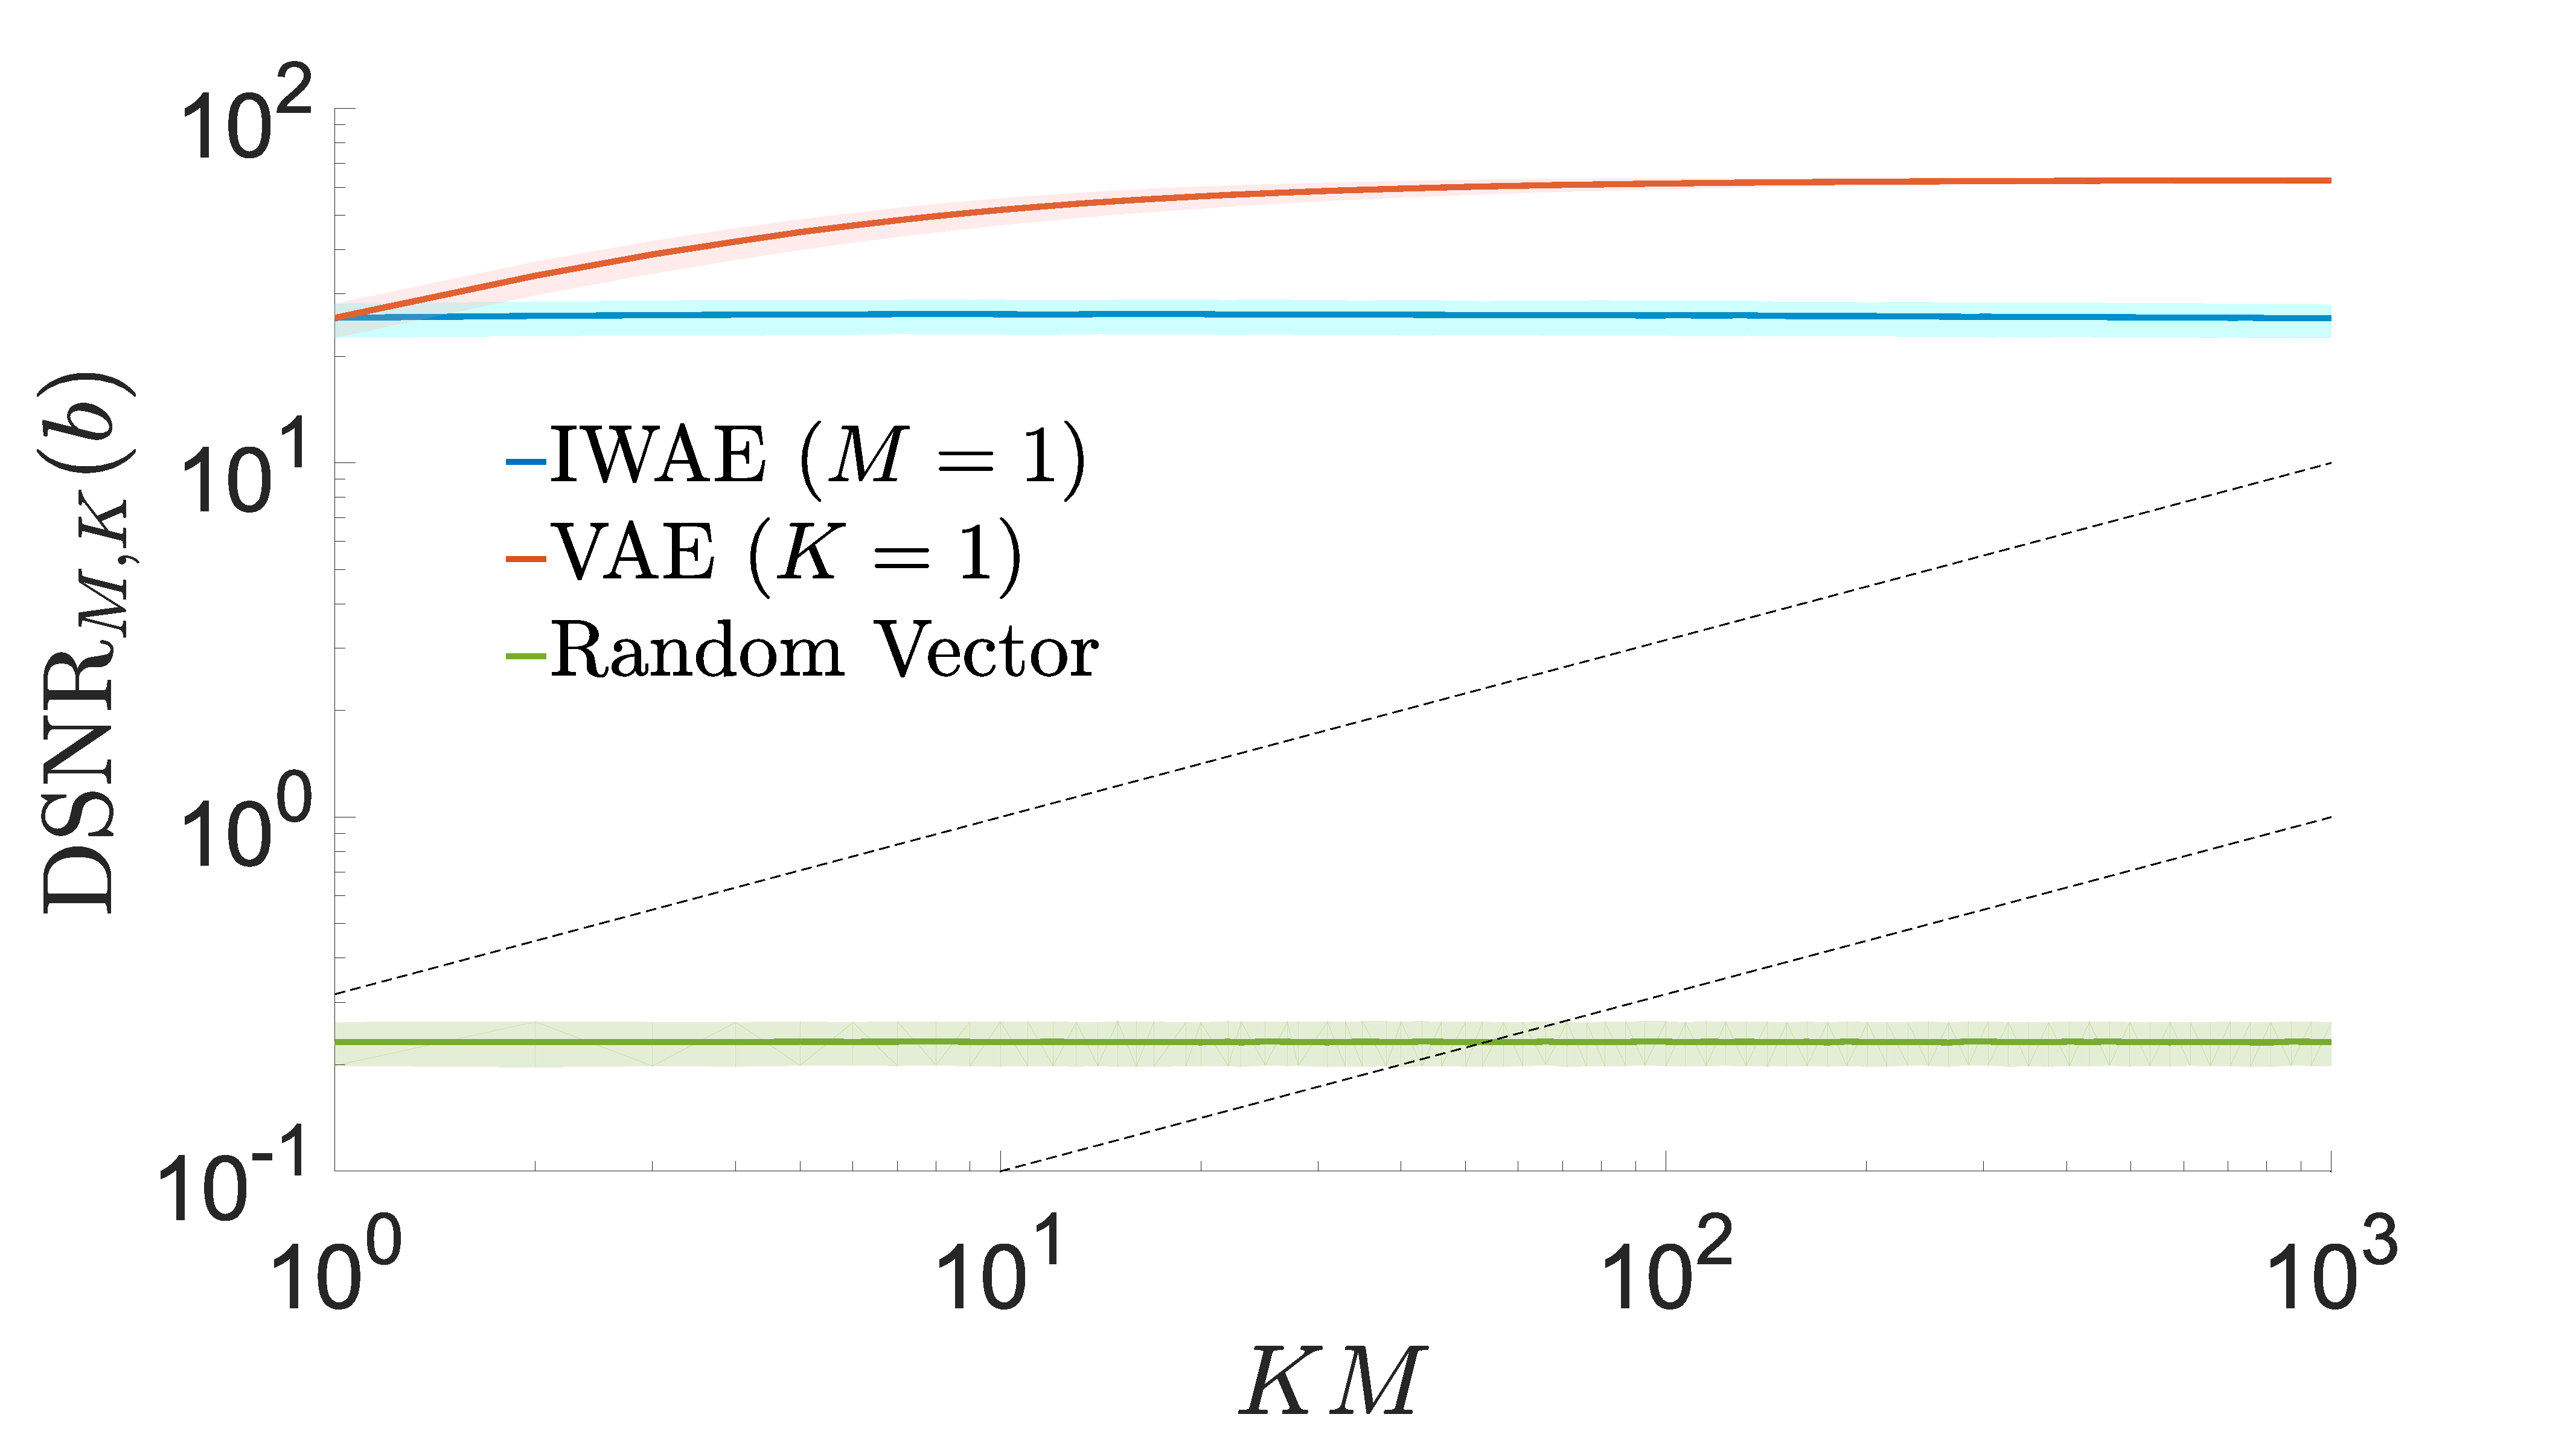
\includegraphics[width=\textwidth]{hv_dir_snr_end}
		\caption{Convergence of \textsc{dsnr} for inference network\label{fig:snr/hv_snr_dir_end}}
	\end{subfigure} ~~~~~~~~~~
	\begin{subfigure}[b]{0.45\textwidth}
		\centering
		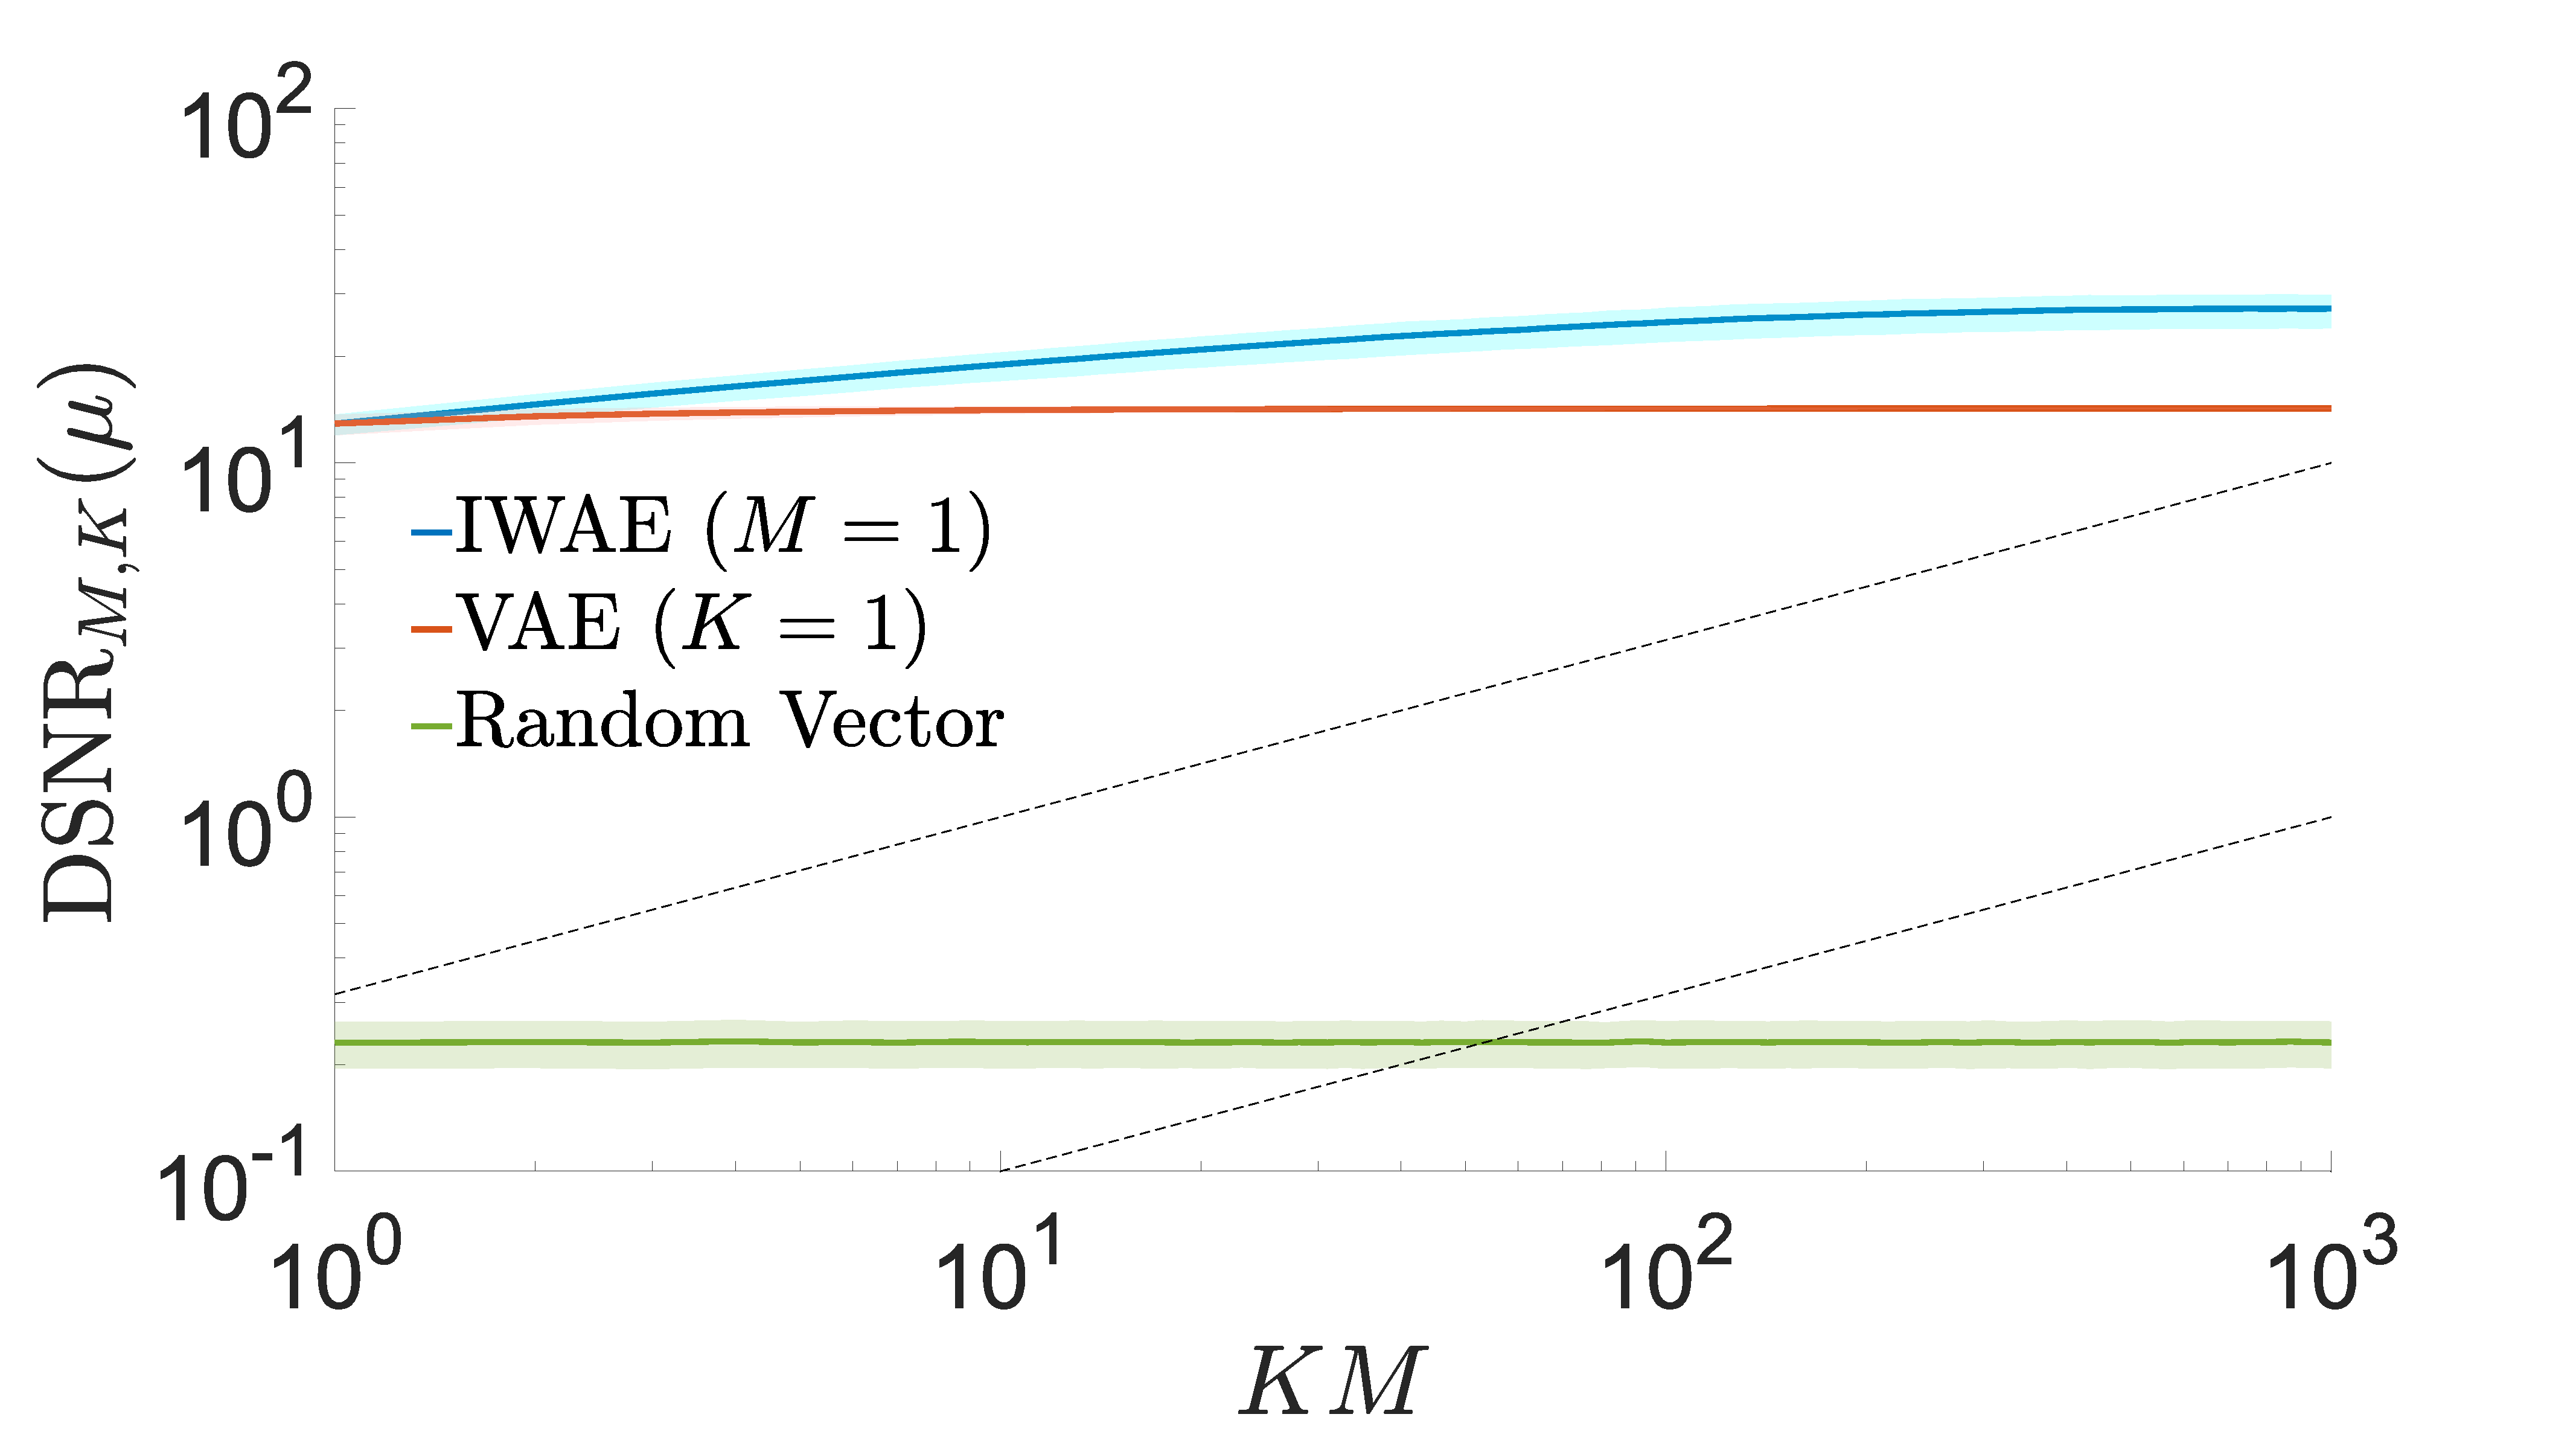
\includegraphics[width=\textwidth]{hv_dir_snr_mu_end}
		\caption{Convergence of \textsc{dsnr} for generative network\label{fig:snr/hv_snr_dir_mu_end}}
	\end{subfigure}
	\caption{Convergence of directional signal-to-noise ratio of gradient estimates where the
		true gradient is taken as $\E \left[\Delta_{1,1000}\right]$ as per
		Figure~\ref{fig:snr/extra_end}.
		\label{fig:snr/hv_extra_end}}
\end{figure}